\documentclass[11pt,oneside]{article}

\usepackage[letterpaper,margin=0.86in,headheight=15pt]{geometry}
\usepackage[T1]{fontenc}
\usepackage[utf8]{inputenc}
\usepackage{lmodern}
\usepackage{microtype}
\usepackage{amsmath,amssymb,amsthm,mathtools,mathrsfs}
\usepackage{bm}
\usepackage{booktabs,longtable,array,tabularx}
\usepackage{enumitem}
\usepackage{graphicx}
\usepackage{caption}
\usepackage{float}
\usepackage{xcolor}
\usepackage{listings}
\usepackage{fancyhdr}
\usepackage{hyperref}
\usepackage[nameinlink,noabbrev]{cleveref}
\usepackage{url}

\definecolor{linkblue}{RGB}{15,76,129}
\definecolor{deepgreen}{RGB}{15,105,67}
\definecolor{deepred}{RGB}{155,34,34}
\definecolor{shade}{RGB}{246,248,250}
\definecolor{rulegray}{RGB}{180,185,190}
\hypersetup{
  colorlinks=true,
  linkcolor=linkblue,
  citecolor=deepgreen,
  urlcolor=linkblue,
  pdftitle={Representations of the Fabius and Rvachev Functions},
  pdfauthor={Research report based on the ProveIt FabiusFunction corpus}
}

\pagestyle{fancy}
\fancyhf{}
\fancyhead[L]{Fabius--Rvachev representation atlas}
\fancyhead[R]{\thepage}
\renewcommand{\headrulewidth}{0.4pt}

\newtheorem{theorem}{Theorem}[section]
\newtheorem{proposition}[theorem]{Proposition}
\newtheorem{corollary}[theorem]{Corollary}
\newtheorem{lemma}[theorem]{Lemma}
\newtheorem{conjecture}[theorem]{Conjecture}
\theoremstyle{definition}
\newtheorem{definition}[theorem]{Definition}
\newtheorem{remark}[theorem]{Remark}
\newtheorem{example}[theorem]{Example}

\newcommand{\dd}{\,\mathrm d}
\newcommand{\e}{\mathrm e}
\newcommand{\ii}{\mathrm i}
\newcommand{\E}{\mathbb E}
\newcommand{\Pp}{\mathbb P}
\newcommand{\R}{\mathbb R}
\newcommand{\C}{\mathbb C}
\newcommand{\N}{\mathbb N}
\newcommand{\Z}{\mathbb Z}
\newcommand{\Up}{\operatorname{up}}
\newcommand{\sinc}{\operatorname{sinc}}
\newcommand{\Tr}{\operatorname{Tr}}
\newcommand{\Spec}{\operatorname{Spec}}
\newcommand{\ord}{\operatorname{ord}}
\newcommand{\vtwo}{\nu_2}
\newcommand{\wt}{s_2}
\newcommand{\bigO}{\mathcal O}
\newcommand{\PhiF}{\Phi}
\newcommand{\phiF}{\varphi}
\newcommand{\Bell}{\mathcal B}
\newcommand{\CorpusKnown}{\textcolor{linkblue}{\textbf{corpus-known}}}
\newcommand{\ProvedHere}{\textcolor{deepgreen}{\textbf{proved here}}}
\newcommand{\DerivedHere}{\textcolor{deepgreen}{\textbf{new operator deduction}}}
\newcommand{\OpenHere}{\textcolor{deepred}{\textbf{conjectural/open}}}

\newenvironment{statusbox}[1]{%
  \par\medskip\begin{center}\begin{minipage}{0.94\textwidth}%
  \hrule\medskip\textbf{#1.}\ }%
  {\par\medskip\hrule\end{minipage}\end{center}\medskip}

\lstdefinestyle{python}{
  language=Python,
  basicstyle=\ttfamily\footnotesize,
  backgroundcolor=\color{shade},
  frame=single,
  rulecolor=\color{rulegray},
  breaklines=true,
  columns=fullflexible,
  keepspaces=true,
  showstringspaces=false,
  keywordstyle=\color{linkblue}\bfseries,
  commentstyle=\color{deepgreen},
  stringstyle=\color{deepred}
}

\title{\bfseries Integral, Series, Product, and Operator Representations\\[0.25em]
for the Fabius--Rvachev System\\[0.6em]
\large A recursive corpus audit, a representation atlas, and new Fredholm,\\
exterior-power, total-positivity, heat-kernel, and Mellin--Barnes bridges}
\author{Research report based on the recursive \texttt{*.tex} corpus under\\
\small\path{Analysis/FabiusFunction/docs}}
\date{27 August 2026\\[0.2em]
\small Audit anchor reported by the repository corpus:\\
\texttt{32d6d36c51d803289e6d6a0dc0c37753766eba47}}

\begin{document}
\maketitle

\begin{abstract}
The Fabius function, Rvachev's compactly supported \(\Up\)-function, their signed
Thue--Morse extension, and their Fourier images admit an unusually dense web of
representations: self-differential and refinement equations, random uniform series,
infinite convolutions, finite box splines, signed truncated-power sums, dyadic sinc and
cosine products, canonical products indexed by the 2-adic valuation, Fourier and
Poisson inversion formulas, cosine and sampling series, moment and cumulant
expansions, exact dyadic composition and \(q\)-binomial formulas, Laplace products,
Mellin transforms, and Lambert-\(W_{-1}\) endpoint coordinates.  This report first
organizes those formulas into a normalization-safe atlas after a recursive audit of the
repository's living references, frozen historical lineages, active frontier drafts, and
transcribed papers.  Results already present in the audited tree are explicitly marked
as such rather than relabeled as discoveries.

The main new contribution relative to the pinned corpus is a specified operator model.
Let \(G=(-\mathrm d^2/\mathrm dx^2)_D^{-1}\) be the Dirichlet Green operator on
\(L^2(0,1)\), and put
\[
 B=\bigoplus_{n\ge1}4^{-n}G.
\]
Then \(B\) is positive trace class and the angular Fourier transform of \(\Up\) is the
Fredholm determinant
\[
 \phiF(t)=\det(I-t^2B).
\]
Equivalently, \(B^{-1}\) has eigenvalues \((2\pi m)^2\) with multiplicity
\(1+\vtwo(m)\).  This specified operator upgrades the scalar ``spectral determinant''
of the existing corpus to a concrete Dirichlet-Laplacian spectrum.  It yields new
resolvent and heat-kernel representations, Brownian-bridge quadratic functionals,
complete-Bernstein structure on the imaginary axis, and a Mellin--Barnes determinant
formula for the endpoint Laplace transform.

A second new bridge identifies normalized even moments with exterior-power traces,
\[
 \frac{\E Z^{2k}}{(2k)!}=\Tr(\wedge^kB),
\]
where \(Z\) has density \(\Up\).  Combining this with the exact reciprocal-dyadic
identity gives the positive spectral formula
\[
 F(2^{-n})=2^{-n(n+1)/2}
 \sum_{k=0}^{\lfloor n/2\rfloor}
 \frac{\Tr(\wedge^kB)}{(n-2k)!}.
\]
Newton identities convert it into finite combinations of
\(\zeta(2j)/(\pi^{2j}(4^j-1))\), hence Bernoulli numbers.  Moreover the sequence
\(\{\E Z^{2k}/(2k)!\}_{k\ge0}\) is a P\'olya-frequency sequence of infinite order;
therefore every Toeplitz minor is nonnegative and strict Newton--Tur\'an inequalities
follow.  High-precision numerical experiments verify the product/trace identity, the
exact dyadic formula, the inequalities, and the Mellin--Barnes integral.  The report
ends with carefully separated conjectures and a research program for Fredholm minors,
operator deformations, inverse-Fabius saddles, derivative-zero statistics, and
formalization.
\end{abstract}

\tableofcontents
\clearpage

\section{Scope, audit boundary, and proof-status discipline}
\label{sec:audit}

\subsection{What was audited}

The requested source boundary is the recursive \texttt{*.tex} tree below
\path{Analysis/FabiusFunction/docs}.  The repository's own most recent audit draft
pins commit \texttt{32d6d36c51d803289e6d6a0dc0c37753766eba47} and records 67
distinct LaTeX paths: five living synthesis/reference documents, thirty-two frozen
historical sources, twenty-three active frontier drafts (including twelve Fourier-decay
dossiers), and seven transcribed or corrected papers~\cite{ReshetnikovRepo}.  The present study used those same lineages and compared the living primary exposition, the consolidated frontier
volume, the active draft families, the archive provenance listings, and the paper-source
folders.  Historical revisions were treated as mathematical lineages rather than as
independent claims.

The most important distinction is between two layers.
\begin{enumerate}[label=(\roman*),leftmargin=2.2em]
\item The living primary exposition records definitions and results aligned with Lean
      declarations: the bounded distribution function \(F\), the compact bump \(\Up\),
      the signed global extension, probability models, Fourier products and inversion,
      exact dyadic arithmetic, and the proved part of the endpoint theory.
\item The non-formalized frontier volume and its descendant reports contain developed
      but not yet fully formalized mathematics: all-order endpoint expansions,
      periodic Mellin corrections, inverse asymptotics, sharp sinc-product decay,
      zero spectra and scalar spectral-determinant formulas, arithmetic rays,
      half-integer sampling, Pascal-weighted hierarchies, \(q\)-Richardson schemes,
      and arbitrary exponent-sequence generalizations.
\end{enumerate}

\begin{statusbox}{Meaning of ``new''}
Throughout this report, ``new'' means absent from the pinned repository corpus after
path, phrase, and formula comparison, and derived or proved in this manuscript.  It is
not a claim of exhaustive worldwide priority.  Classical ingredients are cited, and
open statements are labeled as conjectures.
\end{statusbox}

\subsection{Prior art inside the repository}

The following are treated as \CorpusKnown{} and are used as inputs rather than claimed
as discoveries:
\begin{itemize}[leftmargin=2em]
\item the probability-series model, convolution structure, refinement equations, and
      finite Thue--Morse box-spline approximants;
\item the dyadic sinc product, repeated cosine product, integer zero set, multiplicity
      \(1+\vtwo(m)\), canonical product, zero-count defect, scalar spectral zeta,
      scalar heat trace, local zero jets, and \(q\)-deformations;
\item Fourier inversion, Poisson summation, half-integer cosine/sampling formulas,
      moment, cumulant, Bell-polynomial, and Bernoulli-polynomial identities;
\item exact dyadic values, ordered-composition and path sums, determinant recurrences,
      half-base \(q\)-Pochhammer and Gaussian-binomial formulas, denominator results,
      and interpolation/Richardson transforms;
\item endpoint Laplace products, Mellin harmonic sums, nonconstant logarithmic-periodic
      corrections, the lower Lambert coordinate, all-order asymptotics, and the inverse
      Fabius expansion;
\item Thue--Morse Mahler products, Prouhet cancellation, rarefied sums, and automatic
      sign laws;
\item arbitrary nonnegative exponent sequences and the Pascal-weighted hierarchy as
      scalar products and probability laws.
\end{itemize}

The phrase audit found no counterpart in the principal/current frontier sources for a
specified Fredholm operator built from the Dirichlet Green kernel, Brownian-bridge
quadratic functionals, exterior-power traces, P\'olya-frequency/Toeplitz total
positivity of normalized even moments, or the exact exterior-power formula for
\(F(2^{-n})\).  One audited hierarchy report explicitly warns that its word
``spectral'' refers to the zero divisor and not to the spectrum of a specified operator;
that gap is the starting point of \cref{sec:operator}.

\section{Normalization dictionary and the probability model}
\label{sec:normalization}

Normalization errors are particularly easy here because three Fourier conventions and
three closely related functions occur in the literature.  We fix all conventions at
the outset.

\subsection{The three real functions}

Let \(F\colon\R\to[0,1]\) be the Fabius distribution function, normalized by
\[
 F(x)=0\quad(x\le0),\qquad F(1)=1,
\]
with
\begin{equation}
 F'(x)=2F(2x)\quad(0\le x\le\tfrac12),
 \qquad F(1-x)=1-F(x)\quad(0\le x\le1).
 \label{eq:F-basic}
\end{equation}
Rvachev's compact bump is
\begin{equation}
 \Up(x)=
 \begin{cases}
 F(1-|x|),& |x|\le1,\\
 0,& |x|>1.
 \end{cases}
 \label{eq:up-fold}
\end{equation}
Consequently
\begin{equation}
 F(x)=\Up(x-1)\quad(0\le x\le1),
 \qquad
 F'(x)=2\Up(2x-1).
 \label{eq:F-up}
\end{equation}
The signed global extension is
\begin{equation}
 \mathcal F(x)=\sum_{m\ge0}(-1)^{\wt(m)}\Up(x-2m-1),
 \label{eq:signed-extension}
\end{equation}
where the supports are disjoint apart from endpoints.  It satisfies
\begin{equation}
 \mathcal F'(x)=2\mathcal F(2x).
 \label{eq:global-selfdiff}
\end{equation}
These identities are \CorpusKnown{}; see the classical constructions in
\cite{Fabius1966,Arias1982,Rvachev1990}.

\subsection{Random uniform series}

Let \(U_n\) be independent \(\operatorname{Unif}[0,1]\) variables and let
\(V_n=2U_n-1\), so \(V_n\sim\operatorname{Unif}[-1,1]\).  Define
\begin{equation}
 X=\sum_{n\ge1}2^{-n}U_n,
 \qquad
 Z=2X-1=\sum_{n\ge1}2^{-n}V_n.
 \label{eq:random-series}
\end{equation}
Then
\begin{equation}
 F(x)=\Pp(X\le x),\qquad \Up(x)\dd x=\Pp(Z\in\dd x).
 \label{eq:cdf-density}
\end{equation}
Thus \(F\) is a CDF while \(\Up\) is the density of the centered and rescaled law.
This classical probability representation goes back to the distribution-function viewpoint of
Jessen--Wintner and Fabius~\cite{JessenWintner1935,Fabius1966}.  It simultaneously explains positivity, monotonicity, symmetry,
support, convolution formulas, and positive definiteness of the Fourier transform.
The variance is
\begin{equation}
 \E Z^2=\frac13\sum_{n\ge1}4^{-n}=\frac19.
 \label{eq:variance}
\end{equation}

\subsection{Fourier conventions}

We use the angular transform
\begin{equation}
 \phiF(t)=\int_{-1}^{1}\Up(x)\e^{-\ii tx}\dd x=\E\e^{-\ii tZ},
 \label{eq:angular-transform}
\end{equation}
and the cycles-per-unit transform
\begin{equation}
 \PhiF(z)=\int_{-1}^{1}\Up(x)\e^{-2\pi\ii zx}\dd x=\phiF(2\pi z).
 \label{eq:normalized-transform}
\end{equation}
We write \(\sinc t=\sin t/t\) in angular formulas and explicitly write
\(\sin(\pi z)/(\pi z)\) in normalized formulas.

\section{A representation atlas from the audited corpus}
\label{sec:atlas}

This section is a compact, normalization-consistent synthesis of the principal
representations already developed across the source tree.  Later sections attach new
operator meanings and consequences to this atlas.

\subsection{Refinement and functional-differential forms}

The bump satisfies the two-scale equation
\begin{equation}
 \Up'(x)=2\Up(2x+1)-2\Up(2x-1),
 \label{eq:up-refinement}
\end{equation}
with \(\Up\ge0\), support \([-1,1]\), and integral one.  Integrating or differentiating
\eqref{eq:up-refinement} produces a hierarchy of shifted/scaled formulas; folding by
\eqref{eq:up-fold} recovers \eqref{eq:F-basic}.  On the signed extension,
\eqref{eq:global-selfdiff} removes the two shifts at the price of the Thue--Morse sign
pattern.

A Volterra form useful for repeated integration is
\begin{equation}
 F(x)=\int_0^{2x}F(t)\dd t\qquad(x\ge0),
 \label{eq:volterra-F}
\end{equation}
where the globally signed continuation is understood once \(2x>1\).  Iteration gives
simplex integrals and triangular recurrences for dyadic samples.

\subsection{Infinite convolution and finite box splines}

Let
\[
 b_a(x)=\frac1{2a}\mathbf 1_{[-a,a]}(x).
\]
Then
\begin{equation}
 \Up=b_{1/2}*b_{1/4}*b_{1/8}*\cdots
 \label{eq:infinite-convolution}
\end{equation}
with convergence in every standard sense appropriate to the smooth limiting density.
For the finite sum \(Z_N=\sum_{n=1}^N2^{-n}V_n\), write \(u_N\) for its density and
\(a_N=1-2^{-N}\).  Inclusion--exclusion gives the finite box-spline formula
\begin{equation}
 u_N(x)=\frac{2^{N(N-1)/2}}{(N-1)!}
 \sum_{j=0}^{2^N-1}(-1)^{\wt(j)}
 \left(x+a_N-\frac{j}{2^{N-1}}\right)_+^{N-1}.
 \label{eq:finite-box-spline}
\end{equation}
This makes the Thue--Morse sequence visible before the smooth limit is taken.  It is
also a practical representation for derivatives of order below \(N\), because each
finite approximant is piecewise polynomial.

\subsection{Dyadic sinc and cosine products}

Independence in \eqref{eq:random-series} yields
\begin{equation}
 \boxed{\quad
 \phiF(t)=\prod_{n=1}^{\infty}\sinc\!\left(\frac{t}{2^n}\right),
 \qquad
 \PhiF(z)=\prod_{h=0}^{\infty}
 \frac{\sin(\pi z/2^h)}{\pi z/2^h}.
 \quad}
 \label{eq:sinc-products}
\end{equation}
Using \(\sinc x=\prod_{j\ge1}\cos(x/2^j)\) and counting pairs of scales gives
\begin{equation}
 \phiF(t)=\prod_{r=1}^{\infty}
 \cos\!\left(\frac{t}{2^{r+1}}\right)^r,
 \qquad
 \PhiF(z)=\prod_{r=1}^{\infty}
 \cos\!\left(\frac{\pi z}{2^r}\right)^r.
 \label{eq:cosine-products}
\end{equation}
The scale shift immediately gives the Mahler/refinement identities
\begin{equation}
 \phiF(2t)=\sinc(t)\phiF(t),
 \qquad
 \PhiF(2z)=\frac{\sin(2\pi z)}{2\pi z}\PhiF(z).
 \label{eq:phi-scaling}
\end{equation}

\subsection{Collapsed canonical product and 2-adic multiplicity}

Euler's product for sine collapses all scales onto the positive integers:
\begin{equation}
 \boxed{\quad
 \PhiF(z)=\prod_{m=1}^{\infty}
 \left(1-\frac{z^2}{m^2}\right)^{1+\vtwo(m)}.
 \quad}
 \label{eq:canonical-product}
\end{equation}
Indeed, the factor at scale \(h\) vanishes at an integer \(m\) precisely when
\(2^h\mid m\), so
\begin{equation}
 \ord_{z=\pm m}\PhiF=1+\vtwo(m).
 \label{eq:zero-multiplicity}
\end{equation}
The associated Dirichlet series and exact counting function are
\begin{align}
 \sum_{m\ge1}\frac{1+\vtwo(m)}{m^s}
 &=\frac{\zeta(s)}{1-2^{-s}},\qquad \Re s>1,
 \label{eq:zero-zeta}\\
 \sum_{m=1}^{M}(1+\vtwo(m))
 &=2M-\wt(M).
 \label{eq:zero-count}
\end{align}
All of \eqref{eq:canonical-product}--\eqref{eq:zero-count} are \CorpusKnown{}; the
new point in \cref{sec:operator} is that the same multiplicity becomes the actual
degeneracy of a specified self-adjoint operator.

\subsection{Logarithmic, zeta, and Bernoulli series}

Inside the first zero, \(|t|<2\pi\), logarithmic expansion of
\eqref{eq:canonical-product} gives
\begin{equation}
 \log\phiF(t)
 =-\sum_{j\ge1}\frac{t^{2j}}{j}
 \frac{\zeta(2j)}{\pi^{2j}(4^j-1)}.
 \label{eq:log-trace-series-preview}
\end{equation}
Equivalently, for the moment generating function \(M_Z(s)=\phiF(\ii s)\),
\begin{equation}
 \log M_Z(s)=\sum_{j\ge1}(-1)^{j+1}\frac{s^{2j}}{j}
 \frac{\zeta(2j)}{\pi^{2j}(4^j-1)}.
 \label{eq:mgf-log-series}
\end{equation}
Therefore the even cumulants are
\begin{equation}
 \kappa_{2j}(Z)
 =\frac{2^{2j-1}B_{2j}}{j(2^{2j}-1)},
 \qquad \kappa_{2j+1}(Z)=0.
 \label{eq:cumulants}
\end{equation}
Complete Bell polynomials then give
\begin{equation}
 \E Z^{2n}=\Bell_{2n}(0,\kappa_2,0,\kappa_4,\ldots,0,\kappa_{2n}).
 \label{eq:bell-moments}
\end{equation}
The first values are
\begin{equation}
 \E Z^2=\frac19,\quad
 \E Z^4=\frac{19}{675},\quad
 \E Z^6=\frac{583}{59535},\quad
 \E Z^8=\frac{132809}{32531625}.
 \label{eq:first-moments}
\end{equation}

\subsection{Fourier inversion, cosine series, and sampling}

Because \(\Up\in C_c^\infty(\R)\), its transform is rapidly decreasing on the real
axis, and Fourier inversion is absolutely convergent:
\begin{equation}
 \Up(x)=\frac1{2\pi}\int_{-\infty}^{\infty}
 \e^{\ii tx}\phiF(t)\dd t
 =\frac1\pi\int_0^\infty\cos(tx)\phiF(t)\dd t.
 \label{eq:up-fourier-inversion}
\end{equation}
For \(0<x<1\), the symmetric CDF inversion formula gives
\begin{equation}
 F(x)=\frac12+\frac1\pi\int_0^\infty
 \frac{\sin((2x-1)t)}{t}\phiF(t)\dd t.
 \label{eq:F-sine-inversion}
\end{equation}
The period-two cosine expansion of the compact bump is
\begin{equation}
 \Up(x)=\frac12+
 \sum_{k\ge0}\PhiF\!\left(\frac{2k+1}{2}\right)
 \cos((2k+1)\pi x),\qquad |x|\le1.
 \label{eq:half-integer-cosine}
\end{equation}
Integer Fourier coefficients vanish because of \eqref{eq:zero-multiplicity}, leaving
only half-integers.  Paley--Wiener sampling similarly yields
\begin{equation}
 \PhiF(z)=\frac{\sin(2\pi z)}{2\pi z}+
 \sum_{k\in\Z}\PhiF\!\left(\frac{2k+1}{2}\right)
 \frac{\sin\pi(2z-2k-1)}{\pi(2z-2k-1)},
 \label{eq:shannon}
\end{equation}
with the standard \(L^2\) and locally uniform interpretations.  Half-integer
quadrature and arithmetic-ray refinements are developed extensively in the audited
frontier reports.

\subsection{Endpoint Laplace products}

The moment generating function of \(X\) is
\begin{equation}
 A(z)=\E\e^{zX}
 =\prod_{n\ge1}\frac{\e^{z/2^n}-1}{z/2^n}
 =\e^{z/2}\phiF(\ii z/2).
 \label{eq:A-product}
\end{equation}
The negative Laplace transform
\begin{equation}
 L(s)=\E\e^{-sX}=A(-s)
 =\prod_{n\ge1}\frac{1-\e^{-s/2^n}}{s/2^n}
 =\e^{-s/2}\phiF(\ii s/2)
 \label{eq:L-product}
\end{equation}
obeys
\begin{equation}
 L(2s)=\frac{1-\e^{-s}}{s}L(s).
 \label{eq:L-scaling}
\end{equation}
Writing \(\Lambda(s)=\log L(s)\), the corpus derives the harmonic-sum Mellin transform
\begin{equation}
 \int_0^\infty \Lambda(s)s^{w-1}\dd s
 =\frac{2^w}{1-2^w}\bigl[-\Gamma(w)\zeta(1+w)\bigr],
 \qquad -1<\Re w<0,
 \label{eq:known-Mellin}
\end{equation}
and, after Mellin inversion, the logarithmic-periodic decomposition
\begin{equation}
 \Lambda(s)=-\frac{(\log s)^2}{2\log2}+\frac12\log s
 +P(\log_2s)+E(s),
 \label{eq:endpoint-periodic}
\end{equation}
where \(P\) is nonconstant and one-periodic and \(E\) is rapidly small.  This theory is
\CorpusKnown{}; \cref{sec:MB} derives a Fredholm/Mellin--Barnes representation whose
poles reproduce the same decomposition.

\subsection{Exact reciprocal-dyadic values}

Let \(d_n=\E X^n\).  A central exact identity in the corpus, closely related to the arithmetic formulas of
Arias de Reyna~\cite{Arias2018}, is
\begin{equation}
 \boxed{\quad
 F(2^{-n})=2^{-\binom n2}\frac{d_n}{n!}
 =2^{-\binom n2}[z^n]A(z).
 \quad}
 \label{eq:dyadic-moment}
\end{equation}
Among the many equivalent forms are the positive ordered-composition sum
\begin{equation}
 F(2^{-n})=2^{-\binom n2}
 \sum_{(r_1,\ldots,r_\ell)\vDash n}
 \prod_{j=1}^{\ell}
 \frac1{(2^{r_1+\cdots+r_j}-1)(r_j+1)!},
 \label{eq:ordered-composition}
\end{equation}
Bell-polynomial and lower-Hessenberg determinant forms, and a finite half-base
\(q\)-binomial formula of the shape
\begin{equation}
 F(2^{-n})=\frac{\mathcal N_n}{2^{n^2}(1/2;1/2)_n}.
 \label{eq:q-shape}
\end{equation}
The numerator \(\mathcal N_n\) is an explicit alternating Gaussian-binomial sum with
Thue--Morse inner sums.  The new formula in \cref{sec:exterior-dyadic} replaces these
by a finite positive sum of exterior-power traces of one operator.

\subsection{Endpoint and inverse asymptotics}

For \(L_2=\log2\), the lower-Lambert coordinate
\begin{equation}
 \lambda_n=-\frac1{L_2}W_{-1}(-L_2 2^{-n}),
 \qquad \lambda_n-\log_2\lambda_n=n,
 \label{eq:lambda-n}
\end{equation}
organizes the sharp reciprocal-power asymptotics.  The audited frontier volume gives
\begin{equation}
 \log F(2^{-n})
 =-\frac{L_2}{2}\lambda_n^2
 +\left(1+\frac{L_2}{2}\right)\lambda_n
 -\frac12\log\lambda_n+C_F+\Psi(\lambda_n)+\bigO(n^{-1}),
 \label{eq:sharp-dyadic-asymptotic}
\end{equation}
where \(\Psi\) is smooth, nonconstant, mean-zero, and one-periodic, with explicit
Gamma--zeta Fourier coefficients.  All-order corrections use Bell polynomials.  The
same saddle machinery is inverted to describe \(F^{-1}(y)\) as \(y\downarrow0\).
These results are \CorpusKnown{} and provide the asymptotic benchmark for the new
operator formulas below.

\section{A specified Dirichlet operator and a genuine Fredholm determinant}
\label{sec:operator}

\begin{statusbox}{Status}
The scalar sinc products, canonical product, zero multiplicities, and scalar spectral
zeta in this section are \CorpusKnown{}.  The specified Hilbert space, Dirichlet Green
operator, Fredholm determinant, unitary renormalization, and probabilistic operator
consequences are \ProvedHere{} relative to the pinned corpus.
\end{statusbox}

\subsection{The Green block}

Let
\begin{equation}
 D=-\frac{\mathrm d^2}{\mathrm dx^2},
 \qquad
 \mathcal D(D)=H^2(0,1)\cap H_0^1(0,1),
 \label{eq:Dirichlet-D}
\end{equation}
be the positive Dirichlet Laplacian on \(L^2(0,1)\).  Its normalized eigenfunctions and
eigenvalues are
\begin{equation}
 e_k(x)=\sqrt2\sin(k\pi x),
 \qquad
 De_k=\pi^2k^2e_k,
 \qquad k\ge1.
 \label{eq:D-spectrum}
\end{equation}
The inverse \(G=D^{-1}\) is the positive trace-class integral operator
\begin{equation}
 (Gf)(x)=\int_0^1g(x,y)f(y)\dd y,
 \qquad
 g(x,y)=\min(x,y)-xy,
 \label{eq:Green-kernel}
\end{equation}
with
\begin{equation}
 Ge_k=\frac1{\pi^2k^2}e_k,
 \qquad
 \Tr G^s=\frac{\zeta(2s)}{\pi^{2s}}
 \quad(\Re s>\tfrac12).
 \label{eq:G-zeta}
\end{equation}
The same kernel is the covariance kernel of a standard Brownian bridge; that fact will
be used in \cref{sec:prob-operator}.

\subsection{The dyadic direct sum}

Set
\begin{equation}
 \mathscr H=\bigoplus_{n=1}^{\infty}L^2(0,1),
 \qquad
 B=\bigoplus_{n=1}^{\infty}4^{-n}G.
 \label{eq:B-definition}
\end{equation}
Since
\begin{equation}
 \Tr B=\sum_{n\ge1}4^{-n}\Tr G
 =\frac13\frac{\zeta(2)}{\pi^2}=\frac1{18},
 \label{eq:B-trace}
\end{equation}
\(B\) is positive trace class.  Its nonzero eigenvalues, initially indexed by
\((n,k)\in\N^2\), are
\begin{equation}
 \lambda_{n,k}=\frac{4^{-n}}{\pi^2k^2}.
 \label{eq:B-double-spectrum}
\end{equation}

\begin{theorem}[Specified Fredholm realization]
\label{thm:Fredholm}
For every \(t\in\C\),
\begin{equation}
 \boxed{\quad
 \phiF(t)=\det_{\mathscr H}(I-t^2B).
 \quad}
 \label{eq:Fredholm-phi}
\end{equation}
Equivalently,
\begin{equation}
 \PhiF(z)=\det_{\mathscr H}(I-4\pi^2z^2B).
 \label{eq:Fredholm-Phi}
\end{equation}
Both are ordinary trace-class Fredholm determinants, not zeta-regularized products.
\end{theorem}

\begin{proof}
The Fredholm determinant converges locally uniformly because \(B\) is trace class.
Using \eqref{eq:B-double-spectrum} and Euler's sine product,
\begin{align*}
 \det(I-t^2B)
 &=\prod_{n\ge1}\prod_{k\ge1}
   \left(1-\frac{t^2}{\pi^24^nk^2}\right)\\
 &=\prod_{n\ge1}\frac{\sin(t/2^n)}{t/2^n}
 =\phiF(t).
\end{align*}
The normalized statement follows from \(\PhiF(z)=\phiF(2\pi z)\).
\end{proof}

This result gives an operator interpretation to every coefficient in the logarithmic
series.  For \(|t|<2\pi\),
\begin{equation}
 \log\phiF(t)=\Tr\log(I-t^2B)
 =-\sum_{j\ge1}\frac{t^{2j}}j\Tr B^j,
 \label{eq:operator-log}
\end{equation}
where
\begin{equation}
 \boxed{\quad
 p_j:=\Tr B^j
 =\frac{\zeta(2j)}{\pi^{2j}(4^j-1)}.
 \quad}
 \label{eq:power-traces}
\end{equation}
Thus \eqref{eq:log-trace-series-preview} is literally a trace expansion.

\subsection{A self-adjoint operator whose degeneracies are 2-adic}

Let
\begin{equation}
 \mathscr L=B^{-1}
 =\bigoplus_{n\ge1}4^nD
 \label{eq:L-operator}
\end{equation}
with its natural direct-sum domain.  This is positive self-adjoint with compact
resolvent.  Reindexing \(m=2^{n-1}k\) in \eqref{eq:B-double-spectrum} gives
\begin{equation}
 \Spec(\mathscr L)=
 \bigl\{(2\pi m)^2:m\ge1\bigr\},
 \qquad
 \operatorname{mult}_{(2\pi m)^2}\mathscr L=1+\vtwo(m).
 \label{eq:L-spectrum}
\end{equation}
Indeed, \(m=2^{n-1}k\) is possible for exactly
\(n=1,\ldots,1+\vtwo(m)\).  Therefore
\begin{equation}
 \phiF(t)=\det(I-t^2\mathscr L^{-1})
 =\prod_{m\ge1}\left(1-\frac{t^2}{(2\pi m)^2}\right)^{1+\vtwo(m)}.
 \label{eq:angular-canonical}
\end{equation}
This proves that the 2-adic zero multiplicity is an actual spectral degeneracy, not
merely a multiplicity in a formal zero divisor.

The spectral zeta function of \(\mathscr L\) is
\begin{equation}
 \zeta_{\mathscr L}(s)=\Tr\mathscr L^{-s}
 =\frac{\zeta(2s)}{\pi^{2s}(4^s-1)},
 \qquad \Re s>\frac12,
 \label{eq:L-spectral-zeta}
\end{equation}
which extends meromorphically through the right-hand side.  Its poles at
\(s=\pi\ii k/\log2\), including the collision at \(s=0\), are the operator source of
the logarithmic-periodic oscillations encountered in endpoint asymptotics.

\subsection{Exact renormalization by removing one block}

The dyadic direct sum satisfies the unitary equivalences
\begin{equation}
 4B\simeq G\oplus B,
 \qquad
 \mathscr L\simeq4D\oplus4\mathscr L.
 \label{eq:operator-renormalization}
\end{equation}
Taking determinants in the first identity gives
\begin{align}
 \det(I-4t^2B)
 &=\det(I-t^2G)\det(I-t^2B),\notag\\
 \phiF(2t)&=\sinc(t)\phiF(t),
 \label{eq:det-renormalization}
\end{align}
so the familiar Fourier scaling law is an exact block-decimation identity.  On the
imaginary axis, if
\begin{equation}
 D_B(q)=\det(I+qB),\qquad q\in\C,
 \label{eq:DB}
\end{equation}
then
\begin{equation}
 D_B(4q)=\frac{\sinh\sqrt q}{\sqrt q}\,D_B(q).
 \label{eq:DB-renormalization}
\end{equation}
Equations \eqref{eq:L-scaling} and \eqref{eq:DB-renormalization} are the same
renormalization after
\begin{equation}
 L(s)=\e^{-s/2}D_B(s^2/4).
 \label{eq:L-DB}
\end{equation}

\subsection{Geometric-scale and exponent-sequence operators}
\label{sec:operator-generalization}

The construction is not confined to the classical scale.  Let \(0<q<1\), \(c>0\), and
let \(a_n\in\Z_{\ge0}\) satisfy
\begin{equation}
 \sum_{n\ge0}a_n c^2q^{2n}<\infty.
 \label{eq:exp-summability}
\end{equation}
On a direct sum with \(a_n\) copies of \(L^2(0,1)\) at scale \(n\), put
\begin{equation}
 B_{a,q,c}=\bigoplus_{n\ge0}
 \left(c^2q^{2n}G\right)^{\oplus a_n}.
 \label{eq:general-B}
\end{equation}
Then
\begin{equation}
 \det(I-t^2B_{a,q,c})
 =\prod_{n\ge0}\sinc(cq^nt)^{a_n},
 \label{eq:general-det}
\end{equation}
while
\begin{equation}
 \Tr B_{a,q,c}^{s}
 =\frac{\zeta(2s)}{\pi^{2s}}c^{2s}
 \sum_{n\ge0}a_nq^{2ns}.
 \label{eq:general-zeta}
\end{equation}
For \(a_n\equiv1\), this becomes
\begin{equation}
 \Tr B_{q,c}^{s}
 =\frac{c^{2s}\zeta(2s)}{\pi^{2s}(1-q^{2s})}.
 \label{eq:q-geometric-zeta}
\end{equation}
The classical Fabius--Rvachev operator is \(q=c=1/2\).  Thus the exponent-sequence
Dirichlet series in the audited hierarchy is realized as an honest operator trace.  In
particular, scalar ``zero zeta'' identities become spectral zeta identities whenever
the exponents are nonnegative integers.

\section{Resolvent, heat, theta, and Stieltjes representations}
\label{sec:heat}

\subsection{The logarithmic derivative as a resolvent trace}

For \(t\) away from the zeros of \(\phiF\), differentiating the Fredholm determinant
gives
\begin{equation}
 \frac{\phiF'(t)}{\phiF(t)}
 =-2t\Tr\bigl[B(I-t^2B)^{-1}\bigr].
 \label{eq:resolvent-logderivative}
\end{equation}
Using either spectral indexing yields two complementary partial-fraction forms:
\begin{align}
 \frac{\phiF'(t)}{\phiF(t)}
 &=-2t\sum_{m\ge1}\frac{1+\vtwo(m)}{(2\pi m)^2-t^2},
 \label{eq:valuation-resolvent}\\
 &=\sum_{n\ge1}
 \left[2^{-n}\cot\!\left(\frac{t}{2^n}\right)-\frac1t\right].
 \label{eq:cotangent-resolvent}
\end{align}
Although each bracket in \eqref{eq:cotangent-resolvent} contains \(-1/t\), the bracket
as a whole is \(\bigO(4^{-n})\) on compact sets away from poles, so the series is
locally normally convergent.  Equating \eqref{eq:valuation-resolvent} and
\eqref{eq:cotangent-resolvent} gives a 2-adic cotangent identity:
\begin{equation}
 \sum_{n\ge1}
 \left[2^{-n}\cot\!\left(\frac{t}{2^n}\right)-\frac1t\right]
 =-2t\sum_{m\ge1}\frac{1+\vtwo(m)}{(2\pi m)^2-t^2}.
 \label{eq:cot-valuation-identity}
\end{equation}
This is simultaneously a scale expansion and a spectral resolvent expansion.

For the positive determinant \(D_B(q)\),
\begin{equation}
 \frac{\mathrm d}{\mathrm dq}\log D_B(q)
 =\Tr\bigl[B(I+qB)^{-1}\bigr]
 =\sum_{m\ge1}\frac{1+\vtwo(m)}{(2\pi m)^2+q}.
 \label{eq:Stieltjes-resolvent}
\end{equation}
Thus the logarithmic derivative is the Stieltjes transform of the discrete spectral
measure
\begin{equation}
 \rho=\sum_{m\ge1}(1+\vtwo(m))\,\delta_{(2\pi m)^2}.
 \label{eq:spectral-measure}
\end{equation}

\subsection{Heat trace and dyadic theta series}

Define
\begin{equation}
 H(x)=\Tr\e^{-x\mathscr L}
 =\sum_{n\ge1}\sum_{k\ge1}\e^{-\pi^24^nk^2x}
 =\sum_{m\ge1}(1+\vtwo(m))\e^{-(2\pi m)^2x}.
 \label{eq:heat-trace}
\end{equation}
In terms of Jacobi's theta function
\(\vartheta_3(0,q)=1+2\sum_{k\ge1}q^{k^2}\),
\begin{equation}
 H(x)=\frac12\sum_{n\ge1}
 \left[\vartheta_3(0,\e^{-\pi^24^nx})-1\right].
 \label{eq:theta-heat}
\end{equation}
Removing the first block gives the exact heat renormalization
\begin{equation}
 H(x/4)=\sum_{k\ge1}\e^{-\pi^2k^2x}+H(x).
 \label{eq:heat-renormalization}
\end{equation}
The Mellin transform is
\begin{equation}
 \int_0^\infty x^{s-1}H(x)\dd x
 =\Gamma(s)\frac{\zeta(2s)}{\pi^{2s}(4^s-1)},
 \qquad \Re s>\frac12.
 \label{eq:heat-Mellin}
\end{equation}
This is a theta-integral representation of the spectral zeta and a direct route from
Poisson summation to the endpoint logarithmic period.

\subsection{Exponentials of heat integrals}

The elementary identity
\begin{equation}
 \log(1+q\lambda)=\int_0^\infty
 \frac{1-\e^{-qx}}x\e^{-x/\lambda}\dd x,
 \qquad q\ge0,
 \label{eq:log-heat-elementary}
\end{equation}
can be summed over the spectrum because \(B\) is trace class.

\begin{theorem}[Heat-kernel determinant representations]
\label{thm:heat-det}
For \(q\ge0\),
\begin{equation}
 \boxed{\quad
 \log D_B(q)=\int_0^\infty
 \frac{1-\e^{-qx}}x H(x)\dd x.
 \quad}
 \label{eq:positive-heat-det}
\end{equation}
For \(|t|<2\pi\),
\begin{equation}
 \boxed{\quad
 \log\phiF(t)=-\int_0^\infty
 \frac{\e^{t^2x}-1}{x}H(x)\dd x.
 \quad}
 \label{eq:real-heat-det}
\end{equation}
The latter identity extends by analytic continuation from the disk bounded by the first
zero.
\end{theorem}

\begin{proof}
Apply \eqref{eq:log-heat-elementary} to each eigenvalue \(\lambda_j\) and use monotone
convergence for \(q\ge0\).  Since
\(\sum_j\e^{-x/\lambda_j}=H(x)\), this proves
\eqref{eq:positive-heat-det}.  Replacing \(q\) by \(-t^2\) is justified when
\(t^2<\lambda_1^{-1}=4\pi^2\), and gives \eqref{eq:real-heat-det}.
\end{proof}

Combining \eqref{eq:positive-heat-det} and \eqref{eq:theta-heat} produces the explicit
product--integral--theta representation
\begin{equation}
 \phiF(\ii\sqrt q)=
 \exp\!\left\{
 \frac12\sum_{n\ge1}\int_0^\infty
 \frac{1-\e^{-qx}}x
 \bigl[\vartheta_3(0,\e^{-\pi^24^nx})-1\bigr]\dd x
 \right\}.
 \label{eq:theta-det-combination}
\end{equation}

\subsection{Complete Bernstein structure}
\label{sec:CBF}

Let \(f(q)=\log D_B(q)\) for \(q\ge0\).  From
\eqref{eq:Stieltjes-resolvent},
\begin{equation}
 f'(q)=\int_{(0,\infty)}\frac{\rho(\dd y)}{q+y}
 \label{eq:fprime-Stieltjes}
\end{equation}
with \(\rho\) from \eqref{eq:spectral-measure}.  Hence \(f'\) is a Stieltjes function,
and \(f\) is a complete Bernstein function in the sense of
\cite{SchillingBernstein}.  Equivalently, its L\'evy--Khintchine
representation is exactly \eqref{eq:positive-heat-det}, whose L\'evy density is
\begin{equation}
 \frac{H(x)}x
 =\frac1x\sum_{m\ge1}(1+\vtwo(m))\e^{-(2\pi m)^2x}.
 \label{eq:Levy-density}
\end{equation}
In particular,
\begin{equation}
 (-1)^r f^{(r+1)}(q)
 =r!\sum_j\frac{\lambda_j^{r+1}}{(1+q\lambda_j)^{r+1}}>0,
 \qquad r\ge0.
 \label{eq:Bernstein-signs}
\end{equation}
This supplies an infinite family of monotonicity and convexity inequalities for the
imaginary-axis Fourier transform.

\section{Probability laws generated by the operator}
\label{sec:prob-operator}

The Dirichlet block has an immediate probabilistic meaning that is not visible in the
scalar canonical product.  This section turns the determinant and its reciprocal
powers into Laplace transforms of explicit random series.

\subsection{Brownian-bridge quadratic functionals}

Let \(\beta\) be a standard Brownian bridge on \([0,1]\).  Its Karhunen--Lo\`eve expansion is~\cite{Karhunen1947}
\begin{equation}
 \beta(x)=\sum_{k\ge1}\frac{\xi_k}{\pi k}\sqrt2\sin(\pi kx),
 \qquad \xi_k\stackrel{\mathrm{iid}}{\sim}N(0,1),
 \label{eq:bridge-KL}
\end{equation}
and hence
\begin{equation}
 \int_0^1\beta(x)^2\dd x
 =\sum_{k\ge1}\frac{\xi_k^2}{\pi^2k^2}
 \quad\text{almost surely and in }L^1.
 \label{eq:bridge-L2}
\end{equation}
Take independent bridges \(\beta_n\), \(n\ge1\), and define
\begin{equation}
 Q=\sum_{n\ge1}4^{-n}\int_0^1\beta_n(x)^2\dd x.
 \label{eq:Q-bridge}
\end{equation}
The series converges almost surely because
\(\E Q=\Tr B=1/18\).

\begin{theorem}[Brownian-bridge determinant law]
\label{thm:bridge}
For every \(q\ge0\),
\begin{equation}
 \boxed{\quad
 \E\exp\!\left(-\frac q2Q\right)=D_B(q)^{-1/2}
 =\phiF(\ii\sqrt q)^{-1/2}.
 \quad}
 \label{eq:bridge-det-law}
\end{equation}
Equivalently, after grouping equal eigenvalues,
\begin{equation}
 \frac Q2\ \stackrel{d}=\
 \sum_{m\ge1}\Gamma_m,
 \qquad
 \Gamma_m\sim\operatorname{Gamma}
 \left(\frac{1+\vtwo(m)}2,\frac1{(2\pi m)^2}\right),
 \label{eq:bridge-gamma}
\end{equation}
where the second parameter is the scale and the variables are independent.
\end{theorem}

\begin{proof}
Insert \eqref{eq:bridge-L2} into \eqref{eq:Q-bridge}.  The coefficients of the
independent squares \(\xi_{n,k}^2\) are exactly the eigenvalues
\(\lambda_{n,k}\) of \(B\).  For a standard normal variable,
\(\E\exp(-q\lambda\xi^2/2)=(1+q\lambda)^{-1/2}\).  Multiplication over the spectrum
proves \eqref{eq:bridge-det-law}.  Reindexing by \(m=2^{n-1}k\) collects
\(1+\vtwo(m)\) chi-square degrees of freedom at scale \((2\pi m)^{-2}\), which is
\eqref{eq:bridge-gamma}.
\end{proof}

This result places the Rvachev Fourier image beside classical quadratic-functionals
such as the Cram\'er--von Mises statistic, but with an infinite dyadic tower of
independent bridges.  In particular, every fractional reciprocal power
\(D_B(q)^{-\alpha}\), \(\alpha>0\), is completely monotone: replace each gamma shape
in \eqref{eq:bridge-gamma} by \(\alpha(1+\vtwo(m))\).

\subsection{An exponential series and a generalized gamma convolution}

Let \(E_{n,k}\) be independent unit exponential random variables and set
\begin{equation}
 S=\sum_{n,k\ge1}\lambda_{n,k}E_{n,k}.
 \label{eq:S-exp}
\end{equation}
Again \(\E S=\Tr B<\infty\), so the series converges almost surely.

\begin{proposition}[Reciprocal determinant as a Laplace transform]
\label{prop:exp-det}
For \(q\ge0\),
\begin{equation}
 \boxed{\quad
 \E\e^{-qS}=D_B(q)^{-1}.
 \quad}
 \label{eq:exp-det}
\end{equation}
Moreover,
\begin{equation}
 S\stackrel d=\sum_{m\ge1}Y_m,
 \qquad
 Y_m\sim\operatorname{Gamma}
 \left(1+\vtwo(m),\frac1{(2\pi m)^2}\right)
 \label{eq:S-gamma}
\end{equation}
independently.
\end{proposition}

The cumulants of \(S\) are therefore
\begin{equation}
 \kappa_j(S)=(j-1)!\Tr B^j
 =(j-1)!\frac{\zeta(2j)}{\pi^{2j}(4^j-1)},
 \qquad j\ge1.
 \label{eq:S-cumulants}
\end{equation}
If \(h_j(B)\) denotes the complete homogeneous symmetric function of degree \(j\) in
the eigenvalues of \(B\), then
\begin{equation}
 \frac1{D_B(-q)}=\sum_{j\ge0}h_j(B)q^j,
 \qquad
 \E S^j=j!h_j(B).
 \label{eq:h-complete}
\end{equation}
Thus the determinant simultaneously packages two dual symmetric-function families:
its coefficients are exterior powers, while the reciprocal coefficients are symmetric
powers.

\subsection{A Thorin and heat-measure description}

Equation \eqref{eq:exp-det} shows that \(S\) is a generalized gamma convolution with
discrete Thorin measure
\begin{equation}
 U=\sum_{m\ge1}(1+\vtwo(m))\,\delta_{(2\pi m)^2}.
 \label{eq:Thorin}
\end{equation}
Indeed,
\begin{equation}
 -\log\E\e^{-qS}
 =\int_{(0,\infty)}\log\!\left(1+\frac qy\right)U(\dd y),
 \label{eq:Thorin-log}
\end{equation}
which is the same formula as \eqref{eq:positive-heat-det}.  The L\'evy density
\(H(x)/x\) is therefore not an auxiliary analytic device: it is the L\'evy density of
an explicit infinitely divisible probability law.  This creates a three-way dictionary
\[
 \text{dyadic sinc product}
 \longleftrightarrow
 \text{Dirichlet spectrum}
 \longleftrightarrow
 \text{generalized gamma convolution}.
\]

\section{Exterior powers, exact moments, and reciprocal-dyadic values}
\label{sec:exterior-dyadic}

\subsection{Exterior powers are normalized even moments}

For a positive trace-class operator, the Fredholm determinant has the absolutely
convergent trace-ideal expansion~\cite{SimonTrace,GohbergKrein}
\begin{equation}
 D_B(q)=\det(I+qB)=\sum_{k=0}^{\infty}e_k(B)q^k,
 \qquad
 e_k(B)=\Tr(\wedge^kB).
 \label{eq:det-exterior-expansion}
\end{equation}
On the other hand, by the probability model,
\begin{equation}
 D_B(s^2)=\phiF(\ii s)=\E\e^{sZ}
 =\sum_{k=0}^{\infty}\frac{\E Z^{2k}}{(2k)!}s^{2k}.
 \label{eq:mgf-exterior}
\end{equation}
Comparison proves the following exact identification.

\begin{theorem}[Moment--exterior-power identity]
\label{thm:moment-exterior}
For every \(k\ge0\),
\begin{equation}
 \boxed{\quad
 e_k(B)=\Tr(\wedge^kB)=\frac{\E Z^{2k}}{(2k)!}.
 \quad}
 \label{eq:moment-exterior}
\end{equation}
In particular all exterior-power traces are positive rational numbers.
\end{theorem}

The rationality follows from the power traces
\(p_j=\Tr B^j\), since Euler's evaluation of \(\zeta(2j)\) gives
\begin{equation}
 p_j=\frac{(-1)^{j+1}2^{2j-1}B_{2j}}
 {(2j)!(4^j-1)}\in\mathbb Q_{>0}.
 \label{eq:p-Bernoulli}
\end{equation}
Newton's identities become
\begin{equation}
 ne_n=\sum_{j=1}^{n}(-1)^{j-1}p_j e_{n-j},
 \qquad e_0=1,
 \label{eq:Newton-e}
\end{equation}
and the determinant form is
\begin{equation}
 e_n=\frac1{n!}
 \det\begin{pmatrix}
 p_1&1&0&\cdots&0\\
 p_2&p_1&2&\cdots&0\\
 p_3&p_2&p_1&\ddots&\vdots\\
 \vdots&\vdots&\ddots&\ddots&n-1\\
 p_n&p_{n-1}&\cdots&p_2&p_1
 \end{pmatrix}.
 \label{eq:e-determinant}
\end{equation}
Equivalently, the partition expansion is
\begin{equation}
 e_n=\sum_{\substack{m_1+2m_2+\cdots+nm_n=n}}
 \prod_{j=1}^{n}
 \frac1{m_j!}\left(\frac{(-1)^{j-1}p_j}{j}\right)^{m_j}.
 \label{eq:e-partitions}
\end{equation}
Although signs occur in \eqref{eq:e-partitions}, positivity is transparent from the
spectral sum
\begin{equation}
 e_n=\sum_{j_1<\cdots<j_n}\lambda_{j_1}\cdots\lambda_{j_n}.
 \label{eq:e-spectral-sum}
\end{equation}

The first values are
\begin{equation}
 e_0=1,
 \quad e_1=\frac1{18},
 \quad e_2=\frac{19}{16200},
 \quad e_3=\frac{583}{42865200},
 \quad e_4=\frac{132809}{1311675120000}.
 \label{eq:first-e}
\end{equation}

\subsection{A positive spectral formula for \(F(2^{-n})\)}

The audited corpus supplies \eqref{eq:dyadic-moment}.  The centered variable gives
\begin{equation}
 \E X^n=2^{-n}\E(1+Z)^n
 =2^{-n}\sum_{k=0}^{\lfloor n/2\rfloor}
 \binom n{2k}\E Z^{2k}.
 \label{eq:X-centered-moment}
\end{equation}
Substituting \eqref{eq:moment-exterior} into
\eqref{eq:dyadic-moment} proves the promised exact representation.

\begin{theorem}[Exterior-power formula for reciprocal dyadic values]
\label{thm:dyadic-exterior}
For every integer \(n\ge0\),
\begin{equation}
 \boxed{\quad
 F(2^{-n})=2^{-n(n+1)/2}
 \sum_{k=0}^{\lfloor n/2\rfloor}
 \frac{\Tr(\wedge^kB)}{(n-2k)!}.
 \quad}
 \label{eq:dyadic-exterior}
\end{equation}
Equivalently,
\begin{equation}
 2^{n(n+1)/2}F(2^{-n})
 =[z^n]\e^zD_B(z^2).
 \label{eq:dyadic-coefficient-det}
\end{equation}
\end{theorem}

The formula is a finite positive sum even though each exterior trace is itself an
infinite multiple series.  Combining \eqref{eq:dyadic-exterior} with
\eqref{eq:e-partitions} gives a finite Bernoulli--partition expression:
\begin{equation}
 F(2^{-n})=2^{-n(n+1)/2}
 \sum_{k=0}^{\lfloor n/2\rfloor}\frac1{(n-2k)!}
 \sum_{\substack{m_1+2m_2+\cdots+km_k=k}}
 \prod_{j=1}^{k}
 \frac1{m_j!}
 \left[\frac{(-1)^{j-1}}j
 \frac{\zeta(2j)}{\pi^{2j}(4^j-1)}\right]^{m_j}.
 \label{eq:dyadic-Bernoulli-partition}
\end{equation}
A purely positive multiple-zeta form follows from \eqref{eq:e-spectral-sum}:
\begin{equation}
 F(2^{-n})=2^{-n(n+1)/2}
 \sum_{k=0}^{\lfloor n/2\rfloor}\frac1{(n-2k)!}
 \sum_{j_1<\cdots<j_k}\prod_{r=1}^{k}\lambda_{j_r}.
 \label{eq:dyadic-positive-multiple}
\end{equation}
Here the single index \(j\) may be replaced by either the pair \((a,b)\) with
\(\lambda_{a,b}=4^{-a}/(\pi^2b^2)\), or the collapsed integer index with
multiplicity \(1+\vtwo(m)\).

\begin{table}[H]
\centering
\caption{Exact values produced by \eqref{eq:dyadic-exterior}.}
\label{tab:dyadic-values}
\begin{tabular}{ccl}
\toprule
\(n\)&\(2^{-n}\)&\(F(2^{-n})\)\\
\midrule
0&1&\(1\)\\
1&\(1/2\)&\(1/2\)\\
2&\(1/4\)&\(5/72\)\\
3&\(1/8\)&\(1/288\)\\
4&\(1/16\)&\(143/2073600\)\\
5&\(1/32\)&\(19/33177600\)\\
6&\(1/64\)&\(1153/561842749440\)\\
7&\(1/128\)&\(583/179789679820800\)\\
8&\(1/256\)&\(1616353/704200217922109440000\)\\
\bottomrule
\end{tabular}
\end{table}

\subsection{A contour coefficient representation}

Cauchy's formula applied to \eqref{eq:dyadic-coefficient-det} yields, for any
positively oriented circle \(\gamma\) around the origin,
\begin{equation}
 F(2^{-n})=\frac{2^{-n(n+1)/2}}{2\pi\ii}
 \int_{\gamma}\frac{\e^z\det(I+z^2B)}{z^{n+1}}\dd z.
 \label{eq:dyadic-Cauchy}
\end{equation}
This representation invites saddle-point analysis directly on the Fredholm
determinant.  Its stationary equation is the resolvent equation
\begin{equation}
 1+2z\Tr[B(I+z^2B)^{-1}]-\frac{n+1}{z}=0,
 \label{eq:operator-saddle}
\end{equation}
which is an operator counterpart of the lower-Lambert saddle used in the corpus.

\section{P\'olya-frequency structure and real-zero consequences}
\label{sec:PF}

\subsection{Toeplitz total positivity}

The product
\begin{equation}
 D_B(q)=\prod_{j\ge1}(1+\lambda_jq),
 \qquad \lambda_j>0,
 \qquad \sum_j\lambda_j<\infty,
 \label{eq:DB-positive-product}
\end{equation}
places its coefficient sequence in the classical Aissen--Schoenberg--Whitney--Edrei
class~\cite{ASW1952,Edrei1952,Schoenberg1951}.

\begin{theorem}[P\'olya-frequency theorem for normalized even moments]
\label{thm:PF}
The sequence
\begin{equation}
 a_n=e_n(B)=\frac{\E Z^{2n}}{(2n)!},\qquad n\ge0,
 \label{eq:an-PF}
\end{equation}
is a P\'olya-frequency sequence of infinite order.  Equivalently, every finite minor
of the Toeplitz matrix
\begin{equation}
 T(a)=(a_{j-i})_{i,j\ge0},\qquad a_r=0\ (r<0),
 \label{eq:Toeplitz-a}
\end{equation}
is nonnegative.
\end{theorem}

\begin{proof}
Every finite product \(\prod_{j=1}^{N}(1+\lambda_jq)\) has only real nonpositive
zeros, so its coefficient sequence is PF\(_\infty\).  Since
\(\sum_j\lambda_j<\infty\), the finite products converge locally uniformly to
\(D_B\), and every fixed Toeplitz minor converges to the corresponding minor of
\(T(a)\).  Total positivity is closed under this limit.
\end{proof}

The dual Jacobi--Trudi identity gives more information.  If \(\lambda\) and \(\mu\)
are partitions with \(\mu\subseteq\lambda\), then an appropriate Toeplitz minor is the
skew Schur function
\begin{equation}
 \det\bigl(e_{\lambda'_i-\mu'_j-i+j}(B)\bigr)
 =s_{\lambda/\mu}(\lambda_1,\lambda_2,\ldots)\ge0.
 \label{eq:Schur-minors}
\end{equation}
Through the Frobenius character formula, every such minor is an explicit finite
combination of the power traces \eqref{eq:power-traces}, and hence of Bernoulli
numbers.  This extends the single sequence of moments to an infinite hierarchy of
spectral inequalities.

\subsection{Strict Newton--Tur\'an inequalities}

Newton's inequalities for entire functions of Laguerre--P\'olya type imply strong
log-concavity of the factorially normalized coefficients.

\begin{corollary}[Strict Newton inequalities]
\label{cor:Newton}
For every \(n\ge1\),
\begin{equation}
 \boxed{\quad
 e_n(B)^2>\frac{n+1}{n}e_{n-1}(B)e_{n+1}(B).
 \quad}
 \label{eq:strict-Newton}
\end{equation}
Equivalently, the moment sequence satisfies
\begin{equation}
 \left(\frac{\E Z^{2n}}{(2n)!}\right)^2
 >\frac{n+1}{n}
 \frac{\E Z^{2n-2}}{(2n-2)!}
 \frac{\E Z^{2n+2}}{(2n+2)!}.
 \label{eq:moment-Turan}
\end{equation}
\end{corollary}

Equivalently, after normalizing by \(D_B(1)\), the coefficients are the law of a
countable Bernoulli sum and are ultra-log-concave~\cite{Liggett1997}.
Strictness follows because \(D_B\) has infinitely many nonzero roots; the equality
case of the limiting Newton inequality is the zero-free exponential
\(\e^{cq}\), not the determinant \eqref{eq:DB-positive-product}.  Numerically,
\(e_1^2/(e_0e_2)=50/19\approx2.63158\), while the lower bound is \(2\).

\subsection{Laguerre--P\'olya class and derivative zeros}

The finite determinant truncations are polynomials with real zeros
\(\pm\lambda_j^{-1/2}\).  They converge locally uniformly to \(\phiF\), so
\begin{equation}
 \phiF\in\mathcal{LP},
 \label{eq:phi-LP}
\end{equation}
where \(\mathcal{LP}\) is the Laguerre--P\'olya class.  Therefore every derivative
\(\phiF^{(r)}\) has only real zeros.  At \(t=2\pi m\), differentiation removes one
unit of the known multiplicity until it is exhausted; all remaining derivative zeros
are constrained to the real gaps between the spectral points.  This elementary but
strong consequence is useful for validating numerical Fourier calculations and
motivates \cref{conj:derivative-zeros} below.

The power traces also give Euler--Rayleigh bounds for the first positive zero
\(2\pi\): for every \(j\ge1\),
\begin{equation}
 p_j^{-1/(2j)}<2\pi<\sqrt{\frac{p_j}{p_{j+1}}},
 \qquad
 p_j=\frac{\zeta(2j)}{\pi^{2j}(4^j-1)}.
 \label{eq:Euler-Rayleigh}
\end{equation}
Although the zero is already known exactly, these inequalities illustrate how the
Bernoulli trace data alone recover the spectral edge.

\section{Determinant inversion formulas for \(\Up\) and \(F\)}
\label{sec:det-inversion}

Substitution of the Fredholm determinant into classical inversion formulas produces
representations that involve no unnamed Fourier transform.

\subsection{Real Fourier integrals}

For every \(x\in\R\),
\begin{equation}
 \boxed{\quad
 \Up(x)=\frac1{2\pi}\int_{-\infty}^{\infty}
 \e^{\ii tx}\det(I-t^2B)\dd t
 =\frac1\pi\int_0^\infty\cos(tx)\det(I-t^2B)\dd t.
 \quad}
 \label{eq:up-det-Fourier}
\end{equation}
For \(0<x<1\),
\begin{equation}
 \boxed{\quad
 F(x)=\frac12+\frac1\pi\int_0^\infty
 \frac{\sin((2x-1)t)}t\det(I-t^2B)\dd t.
 \quad}
 \label{eq:F-det-sine}
\end{equation}
The integrands are Schwartz on the real axis, despite the determinant's exponential
type in nonreal directions.  Differentiating \eqref{eq:F-det-sine} recovers
\(F'(x)=2\Up(2x-1)\).

\subsection{Bromwich--Fredholm inversion}

Since \(L(s)=\int_{[0,1]}\e^{-sx}\dd F(x)\), integration by parts gives
\begin{equation}
 \int_0^1\e^{-sx}F(x)\dd x=\frac{L(s)-\e^{-s}}s.
 \label{eq:Laplace-CDF}
\end{equation}
It is often cleaner to invert the measure directly.  At every \(0<x<1\) and any
\(c>0\), the standard Laplace--Stieltjes inversion formula gives
\begin{equation}
 F(x)=\lim_{T\to\infty}\frac1{2\pi\ii}
 \int_{c-\ii T}^{c+\ii T}\frac{\e^{sx}}sL(s)\dd s.
 \label{eq:Bromwich-F}
\end{equation}
Using \eqref{eq:L-DB},
\begin{equation}
 \boxed{\quad
 F(x)=\lim_{T\to\infty}\frac1{2\pi\ii}
 \int_{c-\ii T}^{c+\ii T}
 \frac{\e^{s(x-1/2)}}s\det\!\left(I+\frac{s^2}{4}B\right)\dd s.
 \quad}
 \label{eq:Bromwich-Fredholm-F}
\end{equation}
Similarly, at interior points,
\begin{equation}
 2\Up(2x-1)=\lim_{T\to\infty}\frac1{2\pi\ii}
 \int_{c-\ii T}^{c+\ii T}
 \e^{s(x-1/2)}\det\!\left(I+\frac{s^2}{4}B\right)\dd s.
 \label{eq:Bromwich-up}
\end{equation}
These contour formulas are particularly suited to saddle deformation, because their
phase derivative is the explicit resolvent trace \eqref{eq:Stieltjes-resolvent}.

\subsection{A determinant series on compact subdisks}

Within \(|t|<2\pi\), exponentiating the trace series gives
\begin{equation}
 \det(I-t^2B)=
 \exp\!\left[-\sum_{j\ge1}\frac{p_j}{j}t^{2j}\right]
 =\sum_{n\ge0}(-1)^ne_n(B)t^{2n}.
 \label{eq:det-local-series}
\end{equation}
Substituting the first exponential in \eqref{eq:F-det-sine} is useful after splitting
the Fourier integral at any radius below \(2\pi\); substituting the second gives a
moment/exterior-power expansion of the low-frequency contribution.  This is not a
global termwise Fourier inversion---the Taylor series is local---but it provides
rigorous error-controlled hybrid quadrature when paired with the superpolynomial
decay estimates from the audited Fourier dossiers.

\section{A Mellin--Barnes Fredholm representation of the endpoint transform}
\label{sec:MB}

The corpus's Mellin harmonic-sum analysis and the new determinant model meet in a
particularly direct contour integral.  The bridge is the classical Mellin--Barnes
identity~\cite{FlajoletGourdonDumas1995}:
\begin{equation}
 \log(1+x)=\frac1{2\pi\ii}
 \int_{c-\ii\infty}^{c+\ii\infty}
 \frac{\pi}{u\sin\pi u}x^u\dd u,
 \qquad x>0,\quad0<c<1.
 \label{eq:MB-log}
\end{equation}

\begin{theorem}[Endpoint Mellin--Barnes determinant formula]
\label{thm:MB}
Let \(s>0\) and \(1/2<c<1\).  Then
\begin{equation}
 \boxed{\quad
 \log L(s)=-\frac s2+\frac1{2\pi\ii}
 \int_{c-\ii\infty}^{c+\ii\infty}
 \frac{\pi}{u\sin\pi u}
 \left(\frac{s}{2\pi}\right)^{2u}
 \frac{\zeta(2u)}{4^u-1}\dd u.
 \quad}
 \label{eq:MB-L}
\end{equation}
The integral is absolutely convergent on the vertical line.
\end{theorem}

\begin{proof}
By \eqref{eq:L-DB},
\[
 \log L(s)=-\frac s2+\sum_j\log\left(1+\frac{s^2}{4}\lambda_j\right).
\]
Apply \eqref{eq:MB-log} term by term.  The choice \(c>1/2\) ensures
\(\sum_j\lambda_j^c=\Tr B^c<\infty\), so Fubini's theorem is applicable.  The
spectral trace \eqref{eq:L-spectral-zeta} then gives
\[
 \left(\frac{s^2}{4}\right)^u\Tr B^u
 =\left(\frac{s}{2\pi}\right)^{2u}
 \frac{\zeta(2u)}{4^u-1}.
\]
The factor \(1/\sin\pi u\) supplies exponential decay on vertical lines, while the
remaining factors have at most polynomial growth.
\end{proof}

\subsection{Pole geometry and the periodic endpoint term}

The integrand in \eqref{eq:MB-L} has three kinds of relevant singularities.

\begin{enumerate}[label=(\roman*),leftmargin=2.2em]
\item At \(u=1/2\), the pole of \(\zeta(2u)\) has residue \(s/2\), exactly cancelling
      the explicit term \(-s/2\).
\item At
\begin{equation}
 \tau_k=\frac{\pi\ii k}{\log2},\qquad k\in\Z\setminus\{0\},
 \label{eq:tau-k}
\end{equation}
      the zeros of \(4^u-1\) produce the logarithmic-periodic Fourier modes.
\item At \(u=0\), the collision of the pole of \(1/(4^u-1)\) with the double pole of
      \(\pi/(u\sin\pi u)\) produces a triple pole and hence the quadratic polynomial
      in \(\log s\).
\end{enumerate}

Put \(L_2=\log2\), \(a=\log(2\pi)\), and
\begin{equation}
 C_0=\frac{a^2/2+\zeta''(0)-\pi^2/24}{L_2}-\frac{L_2}{12}.
 \label{eq:C0}
\end{equation}
A Laurent expansion at zero gives the residue
\begin{equation}
 -\frac{(\log s)^2}{2L_2}+\frac12\log s+C_0.
 \label{eq:zero-residue}
\end{equation}
For \(k\ne0\), define
\begin{equation}
 c_k=\frac{\pi\zeta(2\tau_k)}
 {2L_2\,\tau_k\sin(\pi\tau_k)}.
 \label{eq:ck-MB}
\end{equation}
Then \(c_{-k}=\overline{c_k}\), and the exponential size of
\(\sin(\pi\tau_k)\) implies rapid convergence of the real periodic function
\begin{equation}
 P_{\mathrm{MB}}(y)=\sum_{k\ne0}c_k\e^{2\pi\ii ky}.
 \label{eq:P-MB}
\end{equation}
Shifting the contour across the imaginary-axis poles yields, for every \(A>0\),
\begin{equation}
 \boxed{\quad
 \log L(s)=-\frac{(\log s)^2}{2\log2}+\frac12\log s+C_0
 +P_{\mathrm{MB}}\!\left(\log_2\frac{s}{2\pi}\right)
 +\bigO_A(s^{-A}).
 \quad}
 \label{eq:MB-asymptotic}
\end{equation}
The negative integers cause no additional residues: the poles of
\(1/\sin\pi u\) are cancelled by the trivial zeros \(\zeta(2u)=0\).  Formula
\eqref{eq:MB-asymptotic} is the Fredholm-residue version of the corpus-known endpoint
periodicity.  Standard functional-equation manipulations convert
\eqref{eq:ck-MB} to the Gamma--zeta coefficients used in the harmonic-sum derivation.

\begin{remark}[What the contour shift proves]
The contour may be moved to an arbitrary fixed left half-plane, giving a remainder
smaller than every fixed negative power of \(s\).  The numerical data and the original
dyadic product indicate a much sharper exponentially small remainder.  A complete
uniform transseries statement is isolated as \cref{conj:resurgence} rather than being
assumed here.
\end{remark}

\subsection{A second Mellin representation through the heat trace}

Combining \eqref{eq:positive-heat-det} with \eqref{eq:L-DB} gives
\begin{equation}
 \log L(s)=-\frac s2+
 \int_0^\infty\frac{1-\e^{-s^2x/4}}xH(x)\dd x.
 \label{eq:L-heat}
\end{equation}
Inserting \eqref{eq:theta-heat} produces the mixed theta--Laplace integral
\begin{equation}
 \log L(s)=-\frac s2+\frac12\sum_{n\ge1}\int_0^\infty
 \frac{1-\e^{-s^2x/4}}x
 \left[\vartheta_3(0,\e^{-\pi^24^nx})-1\right]\dd x.
 \label{eq:L-theta-integral}
\end{equation}
Taking the Mellin transform in \(s^2/4\) recovers \eqref{eq:MB-L}.  Thus the endpoint
oscillation can be viewed in three equivalent ways: poles of the scale-harmonic Mellin
transform, complex dimensions of the Dirichlet tower, or complex poles of the
Fredholm spectral zeta.

\section{Numerical experiments and reproducibility}
\label{sec:numerics}

The archive contains \texttt{numerical\_experiments.py}, written with detailed
comments and using \texttt{mpmath}, \texttt{sympy}, and \texttt{matplotlib}.  It
regenerates every CSV table and figure in this section.  All transcendental checks use
50 decimal digits; the exact moment and dyadic calculations use rational arithmetic.

\subsection{Fourier product versus trace exponential}

For \(|t|<2\pi\), the code compares
\[
 \prod_{n=1}^{120}\sinc(t/2^n)
 \quad\text{with}\quad
 \exp\!\left(-\sum_{j=1}^{180}\frac{p_jt^{2j}}j\right).
\]
Representative values are shown in \cref{tab:product-check}.

\begin{table}[H]
\centering
\caption{Dyadic product and trace-series agreement.}
\label{tab:product-check}
\begin{tabular}{rrrr}
\toprule
\(t\)&dyadic sinc product&trace exponential&absolute error\\
\midrule
0.25&0.9965323558631412&0.9965323558631412&\(1.6\times10^{-50}\)\\
0.75&0.9691186832108649&0.9691186832108649&\(1.6\times10^{-50}\)\\
1.50&0.8807851433857338&0.8807851433857338&\(9.4\times10^{-51}\)\\
2.75&0.6413734517278066&0.6413734517278066&\(2.3\times10^{-50}\)\\
4.00&0.3617631389237471&0.3617631389237471&\(2.7\times10^{-51}\)\\
5.25&0.1258123621455857&0.1258123621455857&\(1.3\times10^{-31}\)\\
\bottomrule
\end{tabular}
\end{table}
The slower convergence near \(t=5.25\) reflects the radius \(2\pi\) set by the first
spectral zero.

\begin{figure}[H]
\centering
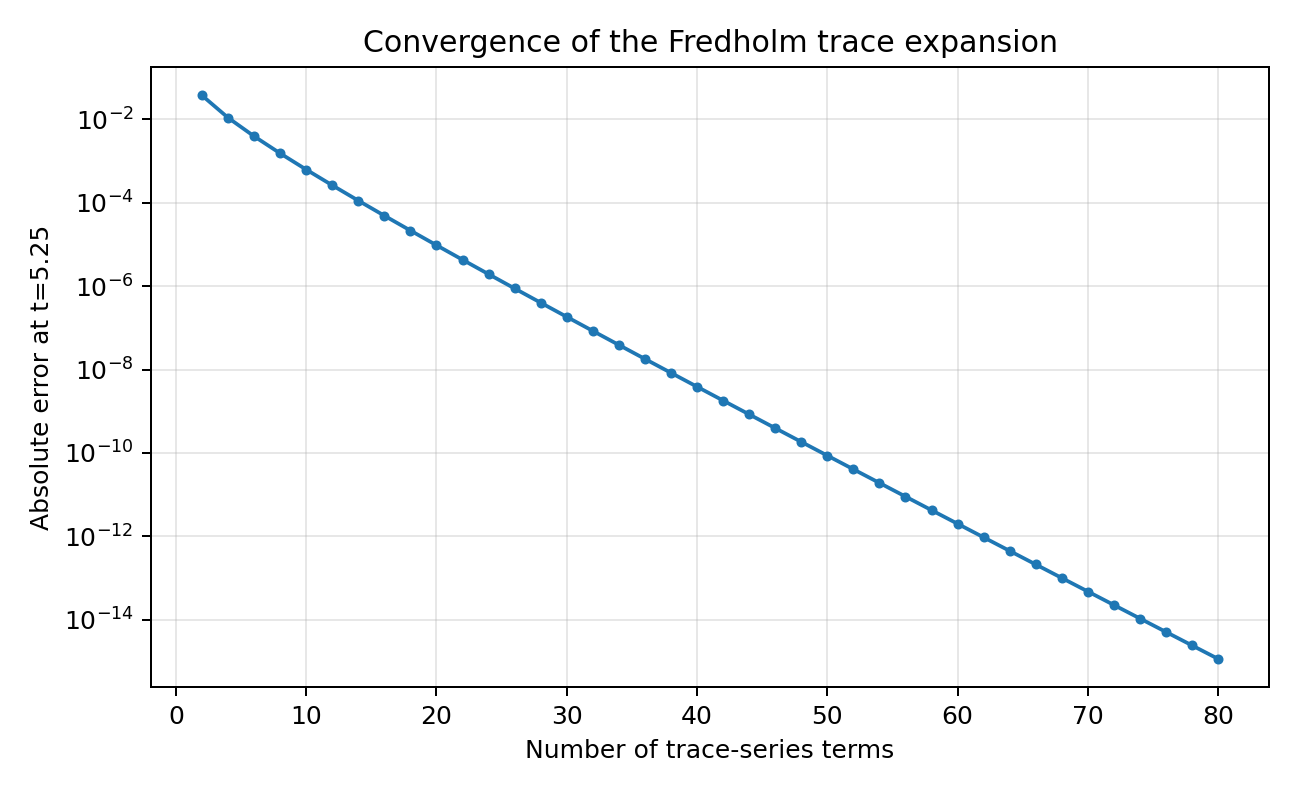
\includegraphics[width=0.78\textwidth]{trace_series_convergence.png}
\caption{Convergence of the trace expansion at \(t=5.25\).}
\label{fig:trace-convergence}
\end{figure}

\subsection{Exact exterior powers and Tur\'an ratios}

Newton's identities were evaluated exactly through \(e_{18}\), and
\eqref{eq:dyadic-exterior} was checked through \(n=15\).  The generated files
\texttt{exterior\_coefficients.csv} and \texttt{dyadic\_exterior\_values.csv} contain
all fractions.  The strict inequality ratio
\begin{equation}
 R_n=\frac{e_n^2}{e_{n-1}e_{n+1}}
 \label{eq:Rn}
\end{equation}
was compared with \((n+1)/n\) for \(1\le n\le14\).  The gaps remain positive and
decrease smoothly, as shown in \cref{fig:turan}.

\begin{figure}[H]
\centering
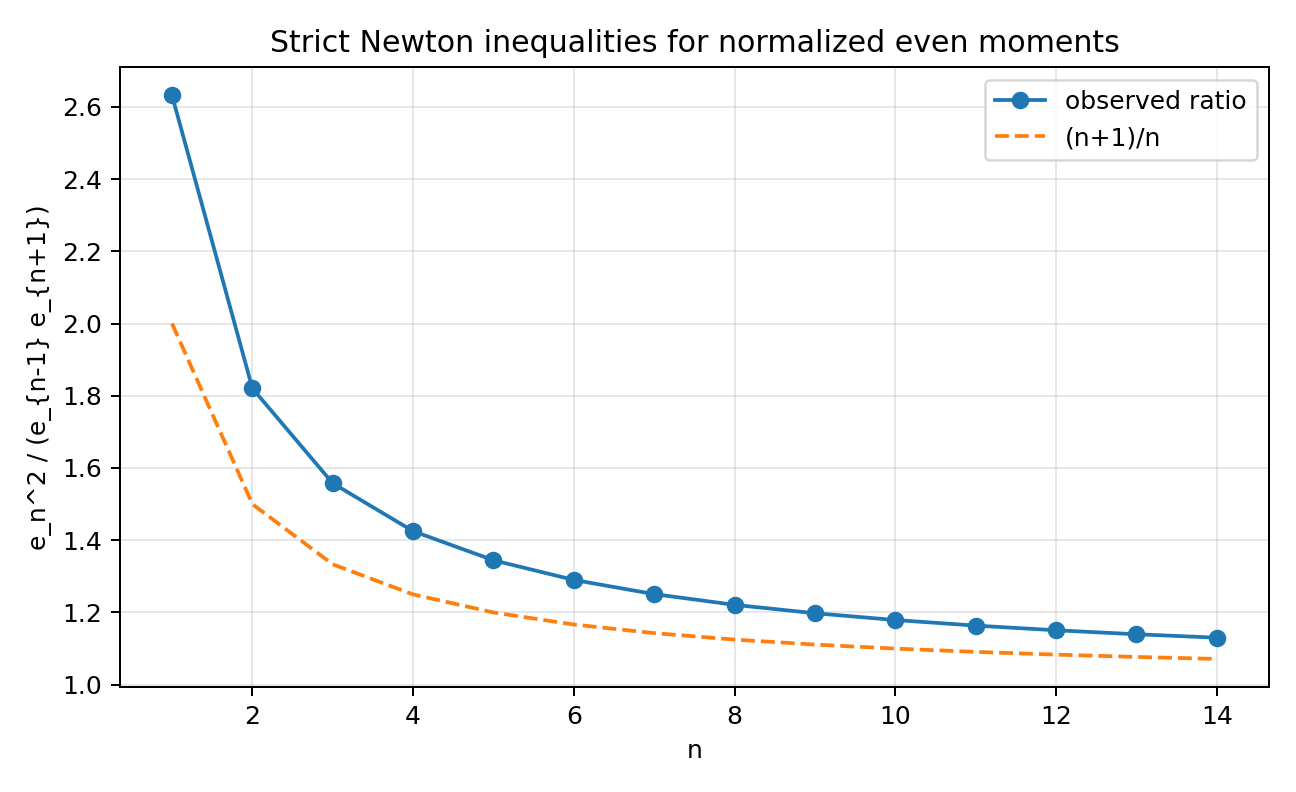
\includegraphics[width=0.78\textwidth]{turan_ratios.png}
\caption{Observed Newton--Tur\'an ratios and the sharp limiting lower bound.}
\label{fig:turan}
\end{figure}

\subsection{Mellin--Barnes validation}

The vertical integral in \eqref{eq:MB-L} was computed on \(\Re u=3/4\), using
conjugation symmetry and a cutoff \(|\Im u|=35\).  Direct evaluation of the endpoint
product and the contour integral agree as follows.

\begin{table}[H]
\centering
\caption{Numerical check of the Mellin--Barnes formula.}
\label{tab:MB-check}
\begin{tabular}{rccc}
\toprule
\(s\)&\(\log L(s)\), product&\(\log L(s)\), MB&absolute error\\
\midrule
0.5&-0.2465292231716876&-0.2465292231716876&\(1.0\times10^{-50}\)\\
2&-0.9448093175660127&-0.9448093175660127&\(1.2\times10^{-50}\)\\
10&-3.782217787719464&-3.782217787719464&\(3.2\times10^{-50}\)\\
50&-10.19248359859169&-10.19248359859169&\(1.7\times10^{-49}\)\\
\bottomrule
\end{tabular}
\end{table}

\begin{figure}[H]
\centering
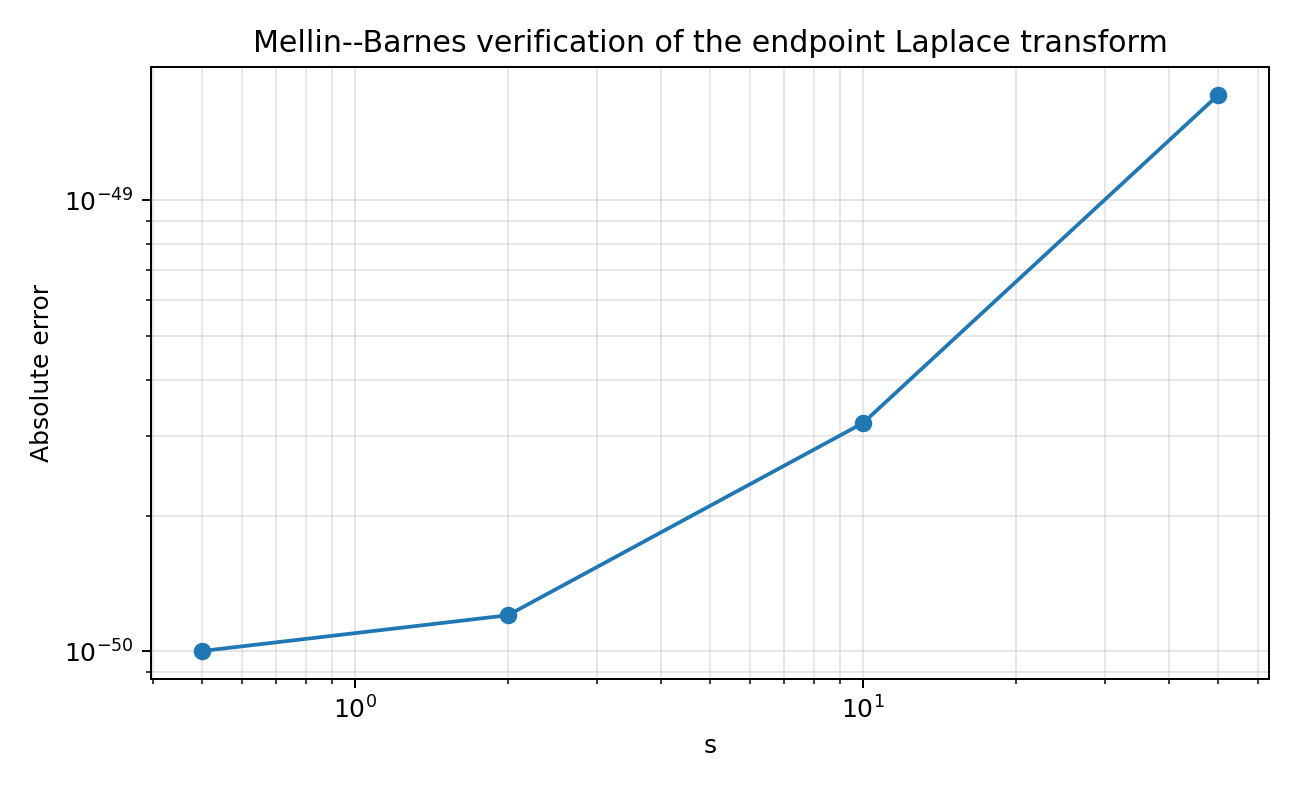
\includegraphics[width=0.78\textwidth]{mellin_barnes_errors.png}
\caption{Absolute errors in the Mellin--Barnes check at 50-digit precision.}
\label{fig:MB-errors}
\end{figure}

The near-machine-precision agreement is not evidence by itself, but it is a useful
independent check of constants, scaling by \(2\pi\), and the cancellation of the
\(u=1/2\) residue.

\section{Further proved deductions and frontier conjectures}
\label{sec:future}

\subsection{A unique critical point in every spectral gap}

The logarithmic derivative can be written symmetrically as
\begin{equation}
 \frac{\phiF'(t)}{\phiF(t)}
 =\sum_{m\ge1}(1+\vtwo(m))
 \left(\frac1{t-2\pi m}+\frac1{t+2\pi m}\right).
 \label{eq:symmetric-logder}
\end{equation}
On each interval \((2\pi m,2\pi(m+1))\), its derivative is strictly negative and its
limits are \(+\infty\) and \(-\infty\).  Hence there is exactly one new zero of
\(\phiF'\) in every positive spectral gap, in addition to the inherited zeros at
\(2\pi m\) of multiplicity \(\vtwo(m)\).  Denote this gap zero by \(c_m\); it is the
unique solution of
\begin{equation}
 \sum_{j\ge1}\frac{1+\vtwo(j)}{c_m^2-(2\pi j)^2}=0,
 \qquad 2\pi m<c_m<2\pi(m+1).
 \label{eq:cm-equation}
\end{equation}
This resolvent characterization appears to be a useful starting point for the finer
question below.

\begin{conjecture}[2-adic modulation of derivative-zero locations]
\label{conj:derivative-zeros}
After subtracting a smooth expansion in descending powers of \(m\), the normalized
gap position
\begin{equation}
 \theta_m=\frac{c_m-2\pi m}{2\pi}\in(0,1)
 \label{eq:theta-m}
\end{equation}
possesses a bounded nonconstant correction determined by the local 2-adic valuation
pattern near \(m\).  More precisely, finite windows of
\((\vtwo(m-r),\ldots,\vtwo(m+r))\) should determine successively accurate
approximations to \(\theta_m\).
\end{conjecture}

\subsection{Fredholm minors for pointwise values}

The determinant inversion formulas represent \(\Up(x)\) and \(F(x)\) by integrals of
a scalar determinant.  A more local operator formula would be stronger.

\begin{conjecture}[A pointwise Fredholm-minor model]
\label{conj:minor}
There exists a natural trace-class integral operator \(K_x\), obtained from the
self-similar Dirichlet tower by a boundary evaluation or rank-one coupling, such that
\(\Up(x)\) on \((-1,1)\) is a Fredholm minor or a ratio of Fredholm determinants of
\(K_x\).  The family can be chosen so that its Schur complement encodes the refinement
equation \eqref{eq:up-refinement}.
\end{conjecture}

A promising construction is to replace the disconnected direct sum by a metric tree
whose edge lengths decrease geometrically and to impose Kirchhoff conditions at the
scale vertices.  The direct-sum spectrum should then appear as the decoupled limit,
while suitable boundary Green functions may recover pointwise values.

\subsection{Operator saddle theory for the inverse Fabius function}

The coefficient saddle \eqref{eq:operator-saddle} and the Bromwich phase derivative
both involve
\begin{equation}
 R(q)=\Tr[B(I+qB)^{-1}]
 =\sum_{m\ge1}\frac{1+\vtwo(m)}{(2\pi m)^2+q}.
 \label{eq:Rq}
\end{equation}
Its complete monotonicity gives robust uniqueness and error bounds for positive
saddles.  This suggests an operator derivation of the lower-Lambert coordinate without
first expanding the scalar product.

\begin{conjecture}[Resolvent-controlled inverse expansion]
\label{conj:inverse-resolvent}
The all-order endpoint expansion of \(F^{-1}(y)\) can be organized entirely in terms
of \(R(q)\) and its derivatives at the unique positive saddle.  After the leading
Lambert inversion, every coefficient is a universal Bell polynomial in the spectral
traces \(\Tr[B^j(I+qB)^{-j}]\), with the logarithmic-periodic component inherited from
the poles of \(\zeta_{\mathscr L}\).
\end{conjecture}

\subsection{Beyond the classical dyadic tower}

The family \eqref{eq:general-B} turns exponent-sequence products into operators, but
several arithmetic questions remain.

\begin{conjecture}[Schur positivity and arithmetic denominators]
\label{conj:Schur-arithmetic}
For the classical spectrum, suitably scaled Schur values
\(s_{\lambda}(\lambda_1,\lambda_2,\ldots)\) have denominator bounds controlled by the
hook lengths of \(\lambda\) and the factors \(2^{2j}-1\) occurring in
\eqref{eq:p-Bernoulli}.  These bounds should refine the known denominator theorems for
\(F(2^{-n})\) when \(\lambda=(1^k)\), and should extend to Pascal-weighted exponent
sequences.
\end{conjecture}

For a geometric ratio \(q\ne1/2\), the spectral zeta denominator
\(1-q^{2s}\) moves the complex dimensions to an arithmetic progression with period
\(|\log q|\).  This makes the operator family a controlled laboratory for separating
features caused by compact convolution from those caused specifically by base two.

\subsection{Exponentially small endpoint structure}

\begin{conjecture}[Resurgent endpoint remainder]
\label{conj:resurgence}
After subtracting the quadratic logarithmic polynomial and the complete periodic
Fourier series in \eqref{eq:MB-asymptotic}, the remainder admits an exponentially
small transseries whose actions are generated by the dyadic semigroup
\(\{j2^r:j,r\in\N\}\).  Its Borel singularities are determined by the factors
\(1-\e^{-s/2^n}\) in \eqref{eq:L-product}, and optimal truncation of the shifted
Mellin--Barnes contour recovers that transseries.
\end{conjecture}

\subsection{Formalization targets}

The most accessible Lean targets are algebraic/operator statements that do not require
the full endpoint saddle machinery:
\begin{enumerate}[leftmargin=2em]
\item construction of finite block operators \(B_N=\bigoplus_{n=1}^N4^{-n}G\) and
      their determinant products;
\item passage to the trace-class limit and proof of \eqref{eq:Fredholm-phi};
\item Newton identities and the finite exact formula \eqref{eq:dyadic-exterior};
\item finite total positivity of the coefficient sequences, followed by stabilization
      of each fixed minor;
\item the resolvent identity \eqref{eq:cot-valuation-identity} on compact subsets away
      from poles.
\end{enumerate}
These steps would turn a substantial part of the new frontier package into a formal
extension of the living repository.

\section{Conclusion}
\label{sec:conclusion}

The Fabius--Rvachev system has no shortage of formulas; the challenge is to organize
them without confusing normalization, proof status, or historical priority.  The
corpus-known representation web begins with a random uniform series and reaches
Thue--Morse splines, sinc and cosine products, 2-adic canonical products, Fourier and
sampling integrals, exact dyadic \(q\)-arithmetic, Mellin harmonic sums, and
Lambert-periodic endpoint asymptotics.

The specified operator
\[
 B=\bigoplus_{n\ge1}4^{-n}(-\mathrm d^2/\mathrm dx^2)_D^{-1}
\]
adds a unifying layer.  Its Fredholm determinant is the Fourier image; its inverse has
2-adic spectral degeneracies; its heat trace gives theta integrals; its resolvent gives
partial fractions and saddle equations; its exterior powers are normalized even
moments; its symmetric powers are moments of an exponential random series; and its
gamma/Brownian laws explain complete monotonicity.  The exact formula
\eqref{eq:dyadic-exterior} connects reciprocal-dyadic Fabius values directly to this
operator, while P\'olya-frequency theory yields a new hierarchy of total-positivity and
Tur\'an inequalities.  Finally, the Mellin--Barnes formula \eqref{eq:MB-L} identifies
the endpoint logarithmic period with the complex dimensions of the same Dirichlet
tower.

These links do not replace the existing \(q\)-binomial, Thue--Morse, Bell, Bernoulli,
or Lambert descriptions.  They explain why those descriptions coexist and supply new
routes between them.  The most promising next step is to develop Fredholm minors and
operator saddles far enough to produce pointwise and inverse-function formulas, then
to formalize the finite-block approximations and their trace-class limit.

\appendix

\section{Master table of representations}
\label{app:atlas}

\small
\begin{longtable}{>{\raggedright\arraybackslash}p{0.15\textwidth}
                  >{\raggedright\arraybackslash}p{0.49\textwidth}
                  >{\raggedright\arraybackslash}p{0.14\textwidth}
                  >{\raggedright\arraybackslash}p{0.12\textwidth}}
\caption{A compact map of the principal representations.}\label{tab:master-atlas}\\
\toprule
Object&type of representation&status&reference\\
\midrule
\endfirsthead
\toprule
Object&type of representation&status&reference\\
\midrule
\endhead
\bottomrule
\endfoot
\(F\)&CDF of \(X=\sum2^{-n}U_n\)&corpus-known&\eqref{eq:cdf-density}\\
\(\Up\)&density of \(Z=\sum2^{-n}V_n\)&corpus-known&\eqref{eq:cdf-density}\\
\(\Up\)&infinite convolution of centered boxes&corpus-known&\eqref{eq:infinite-convolution}\\
\(u_N\)&finite Thue--Morse truncated-power spline&corpus-known&\eqref{eq:finite-box-spline}\\
\(\mathcal F\)&signed translate series and global self-differential equation&corpus-known&\eqref{eq:signed-extension}, \eqref{eq:global-selfdiff}\\
\(\phiF\)&dyadic sinc product&corpus-known&\eqref{eq:sinc-products}\\
\(\phiF\)&multiplicity-weighted cosine product&corpus-known&\eqref{eq:cosine-products}\\
\(\PhiF\)&2-adic canonical product&corpus-known&\eqref{eq:canonical-product}\\
\(\phiF\)&Fredholm determinant of a specified trace-class operator&proved here&\eqref{eq:Fredholm-phi}\\
\(\phiF\)&trace exponential involving \(\zeta(2j)\)&operator form new&\eqref{eq:operator-log}\\
\(\phiF'/\phiF\)&resolvent, valuation partial fractions, and cotangent scales&operator bridge new&\eqref{eq:cot-valuation-identity}\\
\(\phiF(\ii\sqrt q)\)&heat-kernel exponential and theta integral&proved here&\eqref{eq:theta-det-combination}\\
\(D_B^{-1/2}\)&Brownian-bridge quadratic-functional Laplace transform&proved here&\eqref{eq:bridge-det-law}\\
\(D_B^{-1}\)&exponential/gamma random-series Laplace transform&proved here&\eqref{eq:exp-det}, \eqref{eq:S-gamma}\\
\(e_n(B)\)&exterior-power trace and normalized even moment&proved here&\eqref{eq:moment-exterior}\\
\(F(2^{-n})\)&positive finite exterior-power sum&proved here&\eqref{eq:dyadic-exterior}\\
\(F(2^{-n})\)&Cauchy integral of a Fredholm determinant&proved here&\eqref{eq:dyadic-Cauchy}\\
\(\{e_n\}\)&PF\(_\infty\), Toeplitz minors, Schur functions&proved here&\eqref{eq:Toeplitz-a}, \eqref{eq:Schur-minors}\\
\(\Up\)&cosine Fourier determinant integral&operator form new&\eqref{eq:up-det-Fourier}\\
\(F\)&sine Fourier determinant integral&operator form new&\eqref{eq:F-det-sine}\\
\(F\)&Bromwich--Fredholm contour integral&operator form new&\eqref{eq:Bromwich-Fredholm-F}\\
\(L\)&one-sided dyadic product&corpus-known&\eqref{eq:L-product}\\
\(L\)&heat/theta integral&proved here&\eqref{eq:L-heat}, \eqref{eq:L-theta-integral}\\
\(L\)&Mellin--Barnes spectral-zeta integral&proved here&\eqref{eq:MB-L}\\
\(\log L\)&quadratic logarithm plus periodic residue series&new derivation of known structure&\eqref{eq:MB-asymptotic}\\
\(F^{-1}\)&lower-Lambert and periodic saddle expansion&corpus-known&\eqref{eq:lambda-n}, \eqref{eq:sharp-dyadic-asymptotic}\\
\end{longtable}
\normalsize

\section{Proof details for the exterior-power dyadic formula}
\label{app:exterior-proof}

For completeness, the coefficient calculation behind \cref{thm:dyadic-exterior} can
be written in one line.  From \(X=(1+Z)/2\) and symmetry,
\begin{align*}
 [z^n]A(z)
 &=\frac{\E X^n}{n!}
 =\frac1{2^nn!}\sum_{k=0}^{\lfloor n/2\rfloor}
   \binom n{2k}\E Z^{2k}\\
 &=\frac1{2^n}\sum_{k=0}^{\lfloor n/2\rfloor}
   \frac{e_k(B)}{(n-2k)!}.
\end{align*}
Multiplication by \(2^{-\binom n2}\) proves \eqref{eq:dyadic-exterior}.  Equivalently,
\begin{equation}
 A(2z)=\e^z\phiF(\ii z)=\e^zD_B(z^2),
 \label{eq:A2z-det}
\end{equation}
so coefficient extraction immediately gives \eqref{eq:dyadic-coefficient-det}.

The first three nontrivial cases illustrate the mechanism:
\begin{align}
 F(1/4)
 &=2^{-3}\left(\frac1{2!}+e_1\right)
 =\frac18\left(\frac12+\frac1{18}\right)=\frac5{72},
 \label{eq:case-n2}\\
 F(1/8)
 &=2^{-6}\left(\frac1{3!}+e_1\right)
 =\frac1{64}\left(\frac16+\frac1{18}\right)=\frac1{288},
 \label{eq:case-n3}\\
 F(1/16)
 &=2^{-10}\left(\frac1{4!}+\frac{e_1}{2!}+e_2\right)
 =\frac{143}{2073600}.
 \label{eq:case-n4}
\end{align}

\section{Recursive corpus map and nonduplication checklist}
\label{app:corpus}

The repository tree is unusually rich in revisions and parallel frontier reports.  The
audit was therefore conducted by lineage and theorem content rather than by comparing
filenames alone.  The following map records the groups that informed this report.

\begin{longtable}{>{\raggedright\arraybackslash}p{0.23\textwidth}
                  >{\raggedright\arraybackslash}p{0.67\textwidth}}
\toprule
Corpus group&material checked and its role\\
\midrule
\endfirsthead
\toprule
Corpus group&material checked and its role\\
\midrule
\endhead
\bottomrule
\endfoot
Living exposition&Definitions aligned with formal declarations; probability law;
Fourier product and inversion; moments; exact dyadic arithmetic; source-of-truth
normalizations.\\
Mathematical glossary&Notation reconciliation among \(F\), \(\Up\), signed extensions,
Thue--Morse data, \(q\)-products, Bell and Bernoulli polynomials, and Lambert
coordinates.\\
Non-elementarity and Lean walkthroughs&Logical status, proof dependencies, and the
boundary between formalized and research-only statements.\\
Consolidated frontier volume&Endpoint Mellin analysis; logarithmic periodicity;
inverse Fabius asymptotics; Fourier decay; local zero jets; arithmetic rays;
half-integer sampling; integral and interpolation directions.\\
Exponent-sequence/Newton hierarchy&Collapsed multiplicities, zero zeta, scalar
spectral determinant, heat trace, arbitrary exponent sequences, Pascal weighting, and
explicit warning that no operator spectrum was specified.\\
Fourier-decay dossier family&Sharp real-axis bounds, dyadic scale selection,
stationary-scale envelopes, numerical validation, and nonduplication constraints for
new Fourier formulas.\\
Archived revisions&Historical development of exact dyadic, \(q\)-binomial,
Richardson, endpoint, and Thue--Morse results; used to prevent renaming an older result
as new.\\
Transcribed papers&Classical definitions, probability constructions, arithmetic of
dyadic values, and comparison with the independent literature.\\
\end{longtable}

The specific nonduplication checks most relevant to the new results were searches for
operator-defining terms (Fredholm, trace class, Dirichlet Laplacian, Green operator),
probability terms (Brownian bridge, gamma convolution), symmetric-function terms
(exterior power, Schur, P\'olya frequency, total positivity), and the exact spectral
formula \eqref{eq:dyadic-exterior}.  The scalar zero-spectrum material was treated as
prior art throughout.

\section{Numerical archive contents}
\label{app:numerical-files}

The ZIP archive contains the following reproducibility files.

\begin{description}[style=nextline,leftmargin=2.2em]
\item[\texttt{numerical\_experiments.py}]
High-precision product, trace, exact rational, Tur\'an, and Mellin--Barnes checks.  The
script is self-contained apart from the standard Python packages listed in its header.
\item[\texttt{fourier\_product\_trace\_checks.csv}]
Numerical comparison of \eqref{eq:sinc-products} and \eqref{eq:operator-log}.
\item[\texttt{exterior\_coefficients.csv}]
Exact \(e_n(B)\) and \(\E Z^{2n}\) through \(n=18\).
\item[\texttt{dyadic\_exterior\_values.csv}]
Exact values from \eqref{eq:dyadic-exterior} through \(n=15\).
\item[\texttt{turan\_inequalities.csv}]
Ratios in \eqref{eq:strict-Newton} through \(n=14\).
\item[\texttt{mellin\_barnes\_checks.csv}]
Direct-product and vertical-contour values for \eqref{eq:MB-L}.
\item[\texttt{*.png}]
The three figures embedded in \cref{sec:numerics}.
\end{description}

\begin{thebibliography}{99}

\bibitem{Arias1982}
J. Arias de Reyna Mart\'inez,
\emph{Definici\'on y estudio de una funci\'on indefinidamente diferenciable de soporte compacto},
Rev. Real Acad. Cienc. Exact. F\'is. Natur. Madrid \textbf{76} (1982), no.~1, 21--38.
English translation: \url{https://arxiv.org/abs/1702.05442}.

\bibitem{Arias2018}
J. Arias de Reyna,
\emph{Arithmetic of the Fabius function},
Integers \textbf{18} (2018), Paper A51;
\url{https://arxiv.org/abs/1702.06487}.

\bibitem{ASW1952}
M. Aissen, I. J. Schoenberg, and A. M. Whitney,
\emph{On the generating functions of totally positive sequences. I},
J. Analyse Math. \textbf{2} (1952), 93--103.

\bibitem{Edrei1952}
A. Edrei,
\emph{On the generating functions of totally positive sequences. II},
J. Analyse Math. \textbf{2} (1952), 104--109.

\bibitem{Fabius1966}
J. Fabius,
\emph{A probabilistic example of a nowhere analytic \(C^\infty\)-function},
Z. Wahrscheinlichkeitstheorie verw. Gebiete \textbf{5} (1966), 173--174,
\url{https://doi.org/10.1007/BF00536652}.

\bibitem{FlajoletGourdonDumas1995}
P. Flajolet, X. Gourdon, and P. Dumas,
\emph{Mellin transforms and asymptotics: harmonic sums},
Theoret. Comput. Sci. \textbf{144} (1995), 3--58.

\bibitem{GohbergKrein}
I. C. Gohberg and M. G. Kre\u\i n,
\emph{Introduction to the Theory of Linear Nonselfadjoint Operators},
Translations of Mathematical Monographs 18, American Mathematical Society, 1969.

\bibitem{JessenWintner1935}
B. Jessen and A. Wintner,
\emph{Distribution functions and the Riemann zeta function},
Trans. Amer. Math. Soc. \textbf{38} (1935), 48--88,
\url{https://doi.org/10.2307/1989728}.

\bibitem{Karhunen1947}
K. Karhunen,
\emph{\"Uber lineare Methoden in der Wahrscheinlichkeitsrechnung},
Ann. Acad. Sci. Fenn. Ser. A. I. Math.-Phys. \textbf{37} (1947), 1--79.

\bibitem{LevinEntire}
B. Ya. Levin,
\emph{Distribution of Zeros of Entire Functions},
revised edition, Translations of Mathematical Monographs 5, American Mathematical
Society, 1980.

\bibitem{Liggett1997}
T. M. Liggett,
\emph{Ultra logconcave sequences and negative dependence},
J. Combin. Theory Ser. A \textbf{79} (1997), no.~2, 315--325.

\bibitem{ReshetnikovRepo}
V. Reshetnikov,
\emph{ProveIt: FabiusFunction documentation corpus},
recursive LaTeX tree under
\url{https://github.com/VladimirReshetnikov/ProveIt/tree/main/Analysis/FabiusFunction/docs},
accessed 27 August 2026.  Audit anchor reported in the corpus:
\texttt{32d6d36c51d803289e6d6a0dc0c37753766eba47}.

\bibitem{Rvachev1990}
V. A. Rvachev,
\emph{Compactly supported solutions of functional-differential equations and their applications},
Russian Math. Surveys \textbf{45} (1990), no.~1, 87--120,
\url{https://doi.org/10.1070/RM1990v045n01ABEH002324}.

\bibitem{SchillingBernstein}
R. L. Schilling, R. Song, and Z. Vondra\v cek,
\emph{Bernstein Functions: Theory and Applications},
2nd ed., De Gruyter Studies in Mathematics 37, 2012.

\bibitem{Schoenberg1951}
I. J. Schoenberg,
\emph{On P\'olya frequency functions. I. The totally positive functions and their Laplace transforms},
J. Analyse Math. \textbf{1} (1951), 331--374.

\bibitem{SimonTrace}
B. Simon,
\emph{Trace Ideals and Their Applications},
2nd ed., Mathematical Surveys and Monographs 120, American Mathematical Society,
2005.

\bibitem{TitchmarshZeta}
E. C. Titchmarsh,
\emph{The Theory of the Riemann Zeta-Function},
2nd ed., revised by D. R. Heath-Brown, Oxford University Press, 1986.

\end{thebibliography}

\end{document}
